\chapter{Wobbling Motion in Nuclei}

The pioneering work of Bohr and Mottelson \cite{bohr1998nuclear} which was done more than 50 years ago lead to some interesting features regarding the collective phenomena in triaxial nuclei. Namely, they pointed out that a specific precessional motion of the nucleus's spin will take place when the rotational energy is sufficient. The angular momentum for triaxial nuclei is not aligned any of the principal axes of the ellipsoid, but it \emph{precesses} and \emph{wobbles} around one of these axes. They called this phenomenon \textbf{wobbling motion} (w.m.).
This combined motion comes from a consequence regarding the MOI. Indeed, the asymmetry of the three MOI makes the quantum mechanical nature of rotation to be possible around any of the three axes. As such, a \emph{main} rotation around the axis with the largest MOI will be the most energetically favorable, but the other two directions can \emph{quantum mechanically disturb} this main rotation, leading to this unique characteristic of triaxial nuclei.

The non-uniformity nature of w.m. was firstly studied for the `pure' rigid-rotators that correspond to the even-even nuclei. In this case, the w.m. can be treated as small amplitude oscillations of the total angular momentum $\mathbf{I}$ around the axis corresponding to the largest MOI.

\section{Wobbling Motion in Even-Even Nuclei}

The analytical expressions for wobbling excitations were firstly evaluated by Bohr and Mottelson using the so-called \emph{Harmonic Approximation} (HA). This can be described as a small-amplitude limit for the Triaxial Rigid Rotor Hamiltonian that was discussed in Chapter \ref{chapter4} (see Section \ref{trm-model}). In this limit, the projection of the total angular momentum onto the axis with largest MOI can be approximated $I_3\approx I$, meaning that the nucleus will do most of its rotation around this axis, with some `disturbance' from the other two principal of the triaxial rotor. 

For the description of this simple wobbler, one can consider the case when the $3$-axis has the largest MOI, and the following order holds true:
\begin{align}
    \mathcal{I}_3>\mathcal{I}_2>\mathcal{I}_1\ ,
\end{align}
or equivalently:
\begin{align}
    A_3<A_2<A_1\ .
\end{align}
The Hamiltonian can be written as:
\begin{align}
    \hat{H}_\text{rot}={\color{red}A_3I_3^2}+{\color{blue}\left(A_1I_1^2+A_2I_2^2\right)}
    \label{general-rotor-ham-evenA}
\end{align}

The different colors from Eq. \ref{general-rotor-ham-evenA} try to emphasize the fact that a Hamiltonian for the simple wobbler can be regarded as \emph{a main rotation around $3$-axis} (represented by red color) and \emph{the (precession + oscillation) of the total angular momentum} (represented by blue color).

The wobbling excitations which cause oscillations with small amplitudes for $\mathbf{I}$ about the $3$-axis are assumed to have a harmonic-like behavior, meaning that the final energy spectrum of a simple wobbler (even-even nucleus) will have the typical $\hbar\omega(n+1/2)$ behavior. Since this oscillator motion can be explained as `vibrations' of the total angular momentum around a steady position, where each wobbling excitation consists of an additional vibrating phonon, one can express the Hamiltonian in terms of \emph{boson} creation and annihilation operators. As such, the quantum mechanical treatment implies \cite{bohr1998nuclear}:
\begin{align}
    b^\dagger=\frac{1}{\sqrt{2I}}I_+\ ,\ b=\frac{1}{\sqrt{2I}}I_-\ ,\ \left[b,b^\dagger\right]\approx 1\ .
\end{align}

This initial quantization allows one to write Eq. \ref{general-rotor-ham-evenA} as a rotational term and a wobbling-specific one:
\begin{align}
    \hat{H}_\text{rot}&={\color{red}A_3I_3^2}+{\color{blue}H_w}\ ,\label{rot-ham-non-diagonal} \\
    {\color{blue}H_w}&={\color{blue}t_1\left(n+\frac{1}{2}\right)+\frac{1}{2}t_2(b^\dagger b^\dagger + bb)}\ ,
    \label{wob-ham-non-diagonal}
\end{align}
where the \emph{number of boson excitations} is denoted by $n$ and it is given by $n=b^\dagger b$. Each wobbling quanta will carry an angular momentum of one unit less with respect to the $3$-axis. The two factors $t_{1,2}$ are expressed in terms of the inertial parameters as \cite{bohr1998nuclear}:
\begin{align}
    t_1&=I(A_2+A_1-2A_3)\ , \\
    t_2&=I(A_2-A_1)\ .
\end{align}

Notice the linear dependence of the two parameters on the total angular momentum $I$. Moreover, depending on the values of $A_k$, the contribution of $t_{1,2}$ can be negative. Their behavior is shown within the right inset of Fig. \ref{fig-even-even-wobbling-energies}. Although the Hamiltonian $H_w$ is considered to have an oscillator-like behavior, its general expression does not look like a typical harmonic Hamiltonian. For this, the Hamiltonian given in Eq. \ref{wob-ham-non-diagonal} can be brought to a diagonalized form by introducing a new set of boson creation and annihilation operators. These operators will be written as linear combinations of $(b^\dagger,b)$:
\begin{align}
    c^\dagger=w_1b^\dagger-w_2b\ ,\\
    c=w_1b-w_2b^\dagger\ ,
\end{align}
where the two coefficients $w_{1,2}$ are defined in terms of $t_{1,2}$ as:
\begin{align}
    w_1&=\left[\frac{1}{2}\left(\frac{t_1}{\sqrt{t_1^2-t_2^2}}+1\right)\right]^{1/2}\ ,\nonumber\\
    w_2&=\left[\frac{1}{2}\left(\frac{t_1}{\sqrt{t_1^2-t_2^2}}-1\right)\right]^{1/2}\ .
    \label{eqs-w1-w2-terms-wobbling}
\end{align}

The terms $w_{1,2}$ verify the condition $w_1^2-w_2^2=1$ and they make the `dangerous' products ($b^\dagger b^\dagger$,$bb$) disappear in this new representation \cite{oi2006semi}. Note that there is no spin dependence inferred in Eq. \ref{eqs-w1-w2-terms-wobbling} such that $w_{1,2}$ are constant functions of spin, unlike the coefficients $t_{1,2}$. Moreover, introducing a number operator $\hat{n}=c^\dagger c$ and the excitation quanta $\hbar\omega_w$ defined as:
\begin{align}
    \hbar\omega_w=\sqrt{t_1^2-t_2^2}=2I\sqrt{(A_1-A_3)(A_2-A_3)}\ ,
    \label{wobbling-frequency-even-A}
\end{align}
then a final expression of $H_w$ can be expressed, which has a behavior typical to the \emph{harmonic oscillator}:
\begin{align}
    H_w=\hbar\omega_w\left(\hat{n}+\frac{1}{2}\right)\ .
    \label{wob-ham-diagonal}
\end{align}

In this expression, the excitation quanta $\hbar\omega_w$ which was defined in Eq. \ref{wobbling-frequency-even-A} in terms of $t_{1,2}$ is called \emph{wobbling frequency} and its increasing linearly with the total angular momentum. Accordingly, Eq. \ref{rot-ham-non-diagonal} can be re-written with the wobbling Hamiltonian defined in Eq. \ref{wob-ham-diagonal}:
\begin{align}
    \hat{H}_\text{rot}=A_3I(I+1)+\hbar\omega_w\left(\hat{n}+\frac{1}{2}\right)\ .
    \label{rot-wob-ham-diagonal}
\end{align}

Thus, in the HA, the eigenvalues of the rotor Hamiltonian can be expressed in terms of a \emph{wobbling phonon number} $n_w$ (which is the eigenvalue of the number operator $\hat{n}=c^\dagger c$) and a \emph{wobbling frequency} (defined in Eq. \ref{wobbling-frequency-even-A}):
\begin{align}
    E_{I,n}={\color{red}A_3I(I+1)}+{\color{blue}\hbar\omega_w\left(n_w+\frac{1}{2}\right)}\ .
    \label{eq-wobbling-energy-evenA}
\end{align}

The spectrum for an even-even wobbling nucleus is thus represented by Eq. \ref{eq-wobbling-energy-evenA}. Notice again the two colored terms that illustrate the energy coming from the rotation around the $3$-axis and the disturbed motion with small oscillations around the other two axes. Consequently, the wobbling character of the system will be generated by the latter harmonic term. The wobbling phonon number $n_w$ is related to the `strength' of the tilting for $\mathbf{I}$, indicating the fact that an increasing number for $n_w$ will result in oscillations with larger amplitudes around the other two axes. The phonon number takes values $n_w=0,1,\dots$. In inset $b)$ from Fig. \ref{wobbling-geometry-tilting-sketch}, a sketch which shows the tilting effect that the wobbling phonon number has on the total angular momentum vector is drawn. For completeness, the collective structure of two wobbling bands generated through phonon excitations is exemplified in inset $a)$ from Fig. \ref{wobbling-geometry-tilting-sketch}.

\begin{figure}
    \centering
    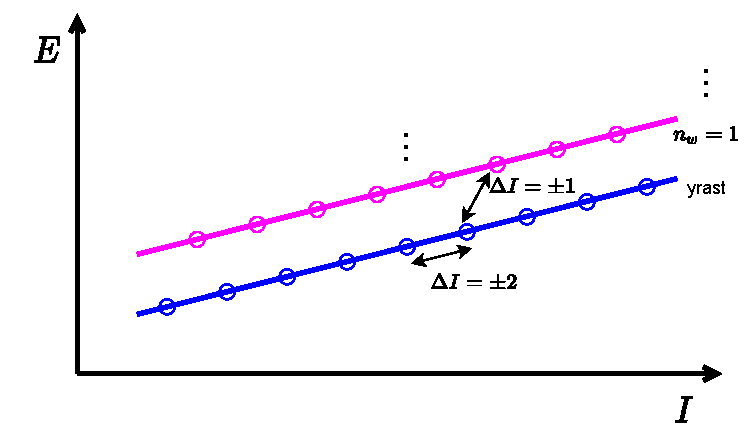
\includegraphics[scale=0.72]{Chapters/Figures/wobbling_n_schematic-1.pdf}
    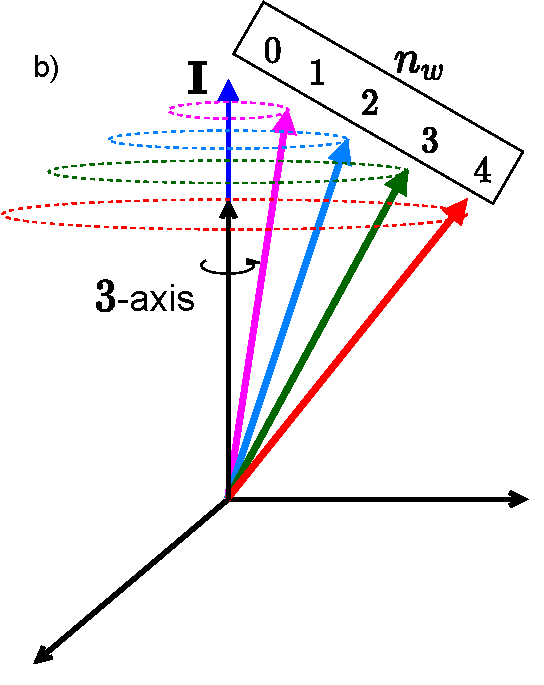
\includegraphics[scale=0.6]{Chapters/Figures/wobbling_n_schematic-2.pdf}
    \caption{\textbf{Left:} A typical wobbling structure for even-even nuclei. The yrast band contains even values of spins since the band has signature $\alpha=0$, while the first excited band has odd spins and $\alpha=1$. The intraband states differ by 2 units of angular momenta, while the interband ones differ with only one unit. \textbf{Right:} The increase of tilting angle between the rotational axis (the $3$-axis in this case) and the total angular momentum $\mathbf{I}$. With each wobbling phonon number, the total angular momentum tilts more and more, generating a `stronger' precessional motion (illustrated by the colored ellipses).}
    \label{wobbling-geometry-tilting-sketch}    
\end{figure}

An alternative way of depicting the wobbling term $H_w$ from Eq. \ref{rot-ham-non-diagonal} would be to express it more generally, in terms of $I_2$ and $I_3$. When doing so, one achieves the following form (assuming that rotation is around the $3$-axis) \cite{oi2006semi}:
\begin{align}
    % H_w={\color{magenta}(A_1-A_3)I_1^2}+{\color{orange}(A_2-A_3)I_2^2}={\color{magenta}T_\text{kin}}+{\color{orange}T_\text{pot}}\ ,
    H_w=(A_1-A_3)I_1^2+(A_2-A_3)I_2^2=T_\text{kin}+T_\text{pot}\ ,
\end{align}
where according to Ref. \cite{wen2015wobbling}, one can regard these two factors as a \emph{kinetic} and a \emph{potential} term. This way of expressing $H_w$ is instructive since it keeps a close contact with the `classical' picture of understanding the total energy of a system.

As a quantitative analysis of the wobbling frequency and the rotor energy, one can take three arbitrary values for the moments of inertia (and, implicitly, the inertia factors $A_k$) and see the behavior of both $E_{I,n}$ and $\hbar\omega_w$ with increasing angular momentum and wobbling phonon number. Keep in mind that depending on the value of the wobbling phonon number, different spin sequences will be allowed. More precisely, from the invariance of the rotor w.r.t. rotations by $\pi$ about the principal axes for even-even nuclei, the signature quantum number $\alpha$ can take the values 0 and 1. Each wobbling band will have an alternating signature, starting with $\alpha=0$ for $n_w=0$ then $\alpha=1$ for $n_w=1$ and so on: even spin sequences appear for even values of $n_w$ and odd spin sequences appear for odd values of $n_w$ (see Fig. \ref{fig-even-even-wobbling-energies}).

The rotor energy from Eq. \ref{eq-wobbling-energy-evenA} is graphically represented for an arbitrary set of moments of inertia as a function of the nuclear angular momentum $I$ in Fig. \ref{fig-even-even-wobbling-energies}. This pedagogical example contains rotational bands up to $n_w=5$ in the wobbling phonon number. From Fig. \ref{fig-even-even-wobbling-energies}, one can see the linear dependence on the total angular momentum and, moreover, the wobbling energy and frequency both are increasing with spin.

\begin{figure}
    \centering
    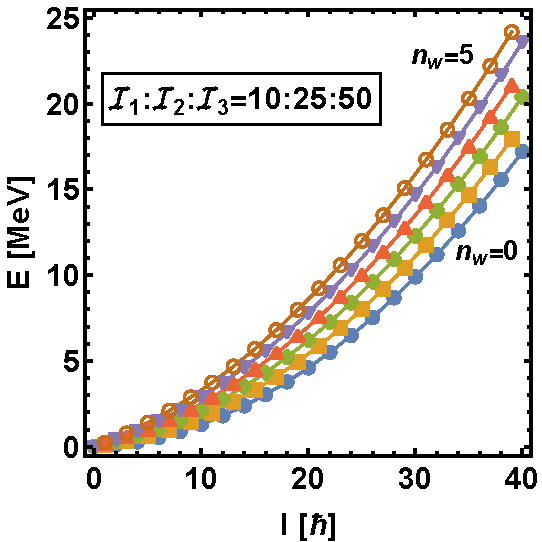
\includegraphics[scale=0.7]{Chapters/Figures/wobbling-evenA.pdf}
    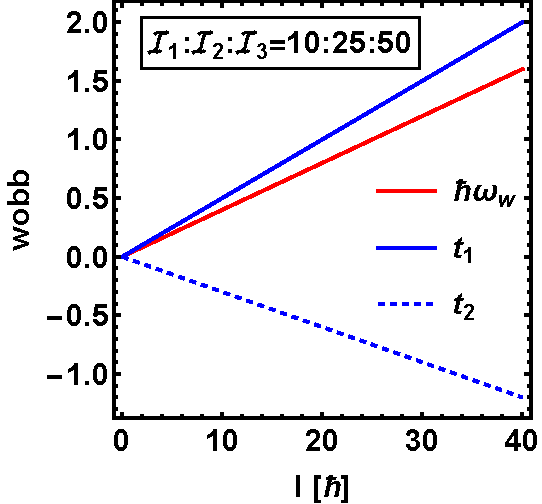
\includegraphics[scale=0.74]{Chapters/Figures/wobblingFreq-evenA.pdf}
    \caption{\textbf{Left:} The energy spectrum for an even-even nucleus with three different moments of inertia, with the main rotation around the $3$-axis, according to Eq. \ref{eq-wobbling-energy-evenA}. Each wobbling band has alternating signature number $\alpha$ (starting with $\alpha=0$ for the ground state $n_w=0$ band). Notice the even/odd spin sequences for each band. \textbf{Right:}: The wobbling frequency plotted together with the linear terms $t_1$ and $t_2$ that are used to express $\hbar\omega_w$. Same set of MOI were used across both figures and the unit for $\mathcal{I}_i$ is $\hbar^2\ \text{MeV}^{-1}$.}
    \label{fig-even-even-wobbling-energies}
\end{figure}


Another instructive analysis would be the evolution of the components of $\mathbf{I}$ as functions of the polar and azimuthal angles $\theta,\varphi$. Indeed, expressing the three angular momentum components as:
\begin{align}
    I_1&=I'\sin\theta\cos\varphi\ ,\\
    I_2&=I'\sin\theta\sin\varphi\ ,\\
    I_3&=I'\cos\theta\ ,
    \label{angular-momentum-polar-components}
\end{align}
where $I'=\sqrt{I(I+1)}$, one can make a graphical representation for them, by letting $\theta$ and $\varphi$ vary within their corresponding intervals. In Fig. \ref{figs-angular-momentum-components-polar}, the quantities $I_1$ and $I_2$ are represented in the $(\theta,\varphi)$ plane for a fixed spin value $I=10\hbar$. Since the third component is independent of the azimuthal angle $\varphi$, it has been dismissed.

\begin{figure}
    \centering
    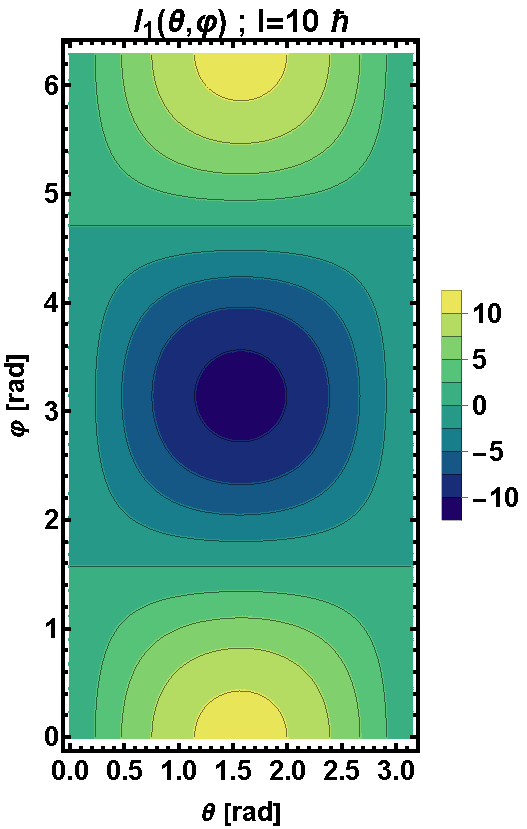
\includegraphics[scale=0.66]{Chapters/Figures/angular_components-TRM-1.pdf}
    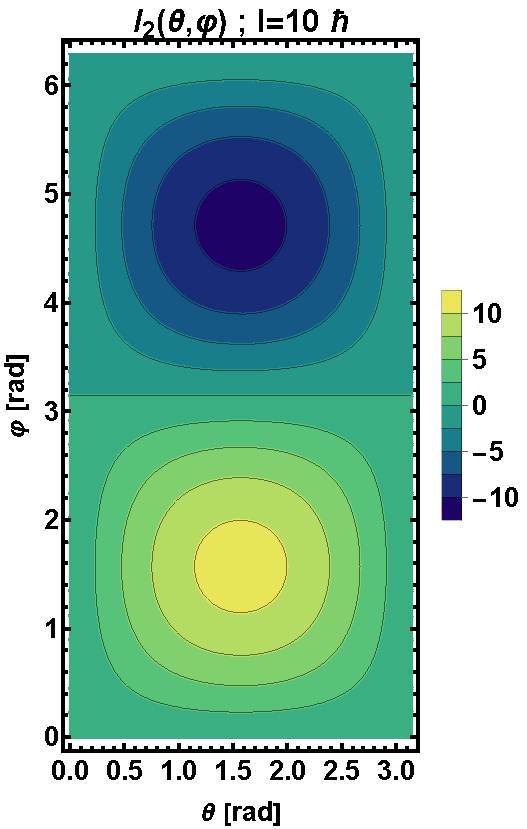
\includegraphics[scale=0.66]{Chapters/Figures/angular_components-TRM-2.pdf}
    \caption{The geometrical representation of the first and second component of the total angular momentum $\mathbf{I}$ as functions of the polar angles, according to Eq. \ref{angular-momentum-polar-components}.}
    \label{figs-angular-momentum-components-polar}
\end{figure}

The other relevant observables that can be calculated for simple wobbler within the HA are the two quadrupole moments $Q_{20,22}$ and the intraband + interband $B(E2)$ transition probabilities. The quadrupole components are expressed in terms of the intrinsic quadrupole moment $Q_0$ and the triaxiality parameter as \cite{shoji2006microscopic}:
\begin{align}
    Q_{20}=Q_0\cos\gamma\ ,\ Q_{22}=\frac{1}{\sqrt{2}}Q_0\sin\gamma\ .
    \label{quadrupole-components-q20-q22}
\end{align}

These components can be furthermore used to determine the intraband $B(E2)$ transition probabilities \cite{wen2015wobbling}:
\begin{align}
    B(E2;(n,I)\to(n,I-2))=\frac{5}{16\pi}Q_{22}^2\ ,
    \label{intraband-probability-simple-wobbler}
\end{align}
and also the interband transitions:
\begin{align}
    B(E2;(n,I)\to(n-1,I-1))&=\frac{5}{16\pi}\frac{n}{I}\left(\sqrt{3}Q_{20}w_1+\sqrt{2}Q_{22}w_2\right)^2\ , \label{interband-probability-simple-wobbler-1}\\
    B(E2;(n,I)\to(n+1,I-1))&=\frac{5}{16\pi}\frac{n+1}{I}\left(\sqrt{3}Q_{20}w_2+\sqrt{2}Q_{22}w_1\right)^2\ .
    \label{interband-probability-simple-wobbler-2}
\end{align}

Notice that for the intraband transitions, going from the state $I$ to $I-2$ will only depend in a quadratic manner on the quadrupole component $Q_{22}$, making thus the transitions spin-independent.

\subsubsection*{Triaxial rotor energy vs. wobbling energy}

An important discussion should be made regarding the nomenclature for energies when referring to wobbling motion. As shown in Eq. \ref{eq-wobbling-energy-evenA}, the energy spectrum for a simple wobbler can be determined for every phonon number and spin sequences. However, that is the `full' spectrum  of the wobbler, which is composed of the \emph{yrast} states with $n_w=0$ and the \emph{excited states} having $n_w=1,\dots$ and so on. On the other hand, the so-called \emph{wobbling energies} are defined in terms of these `absolute values' (i.e., $E_{I,n}$) with the following rules \cite{wen2015wobbling}:
\begin{align}
    E_\text{wob}(I_\text{even})&=E_{I,n}-E_{I,0}\ ,\\
    % E_\text{wob}(I_\text{even})&=E_{I,n}-E_{I,0}\ ,\nonumber \\
    E_\text{wob}(I_\text{odd})&=E_{I,n}-\frac{1}{2}\left(E_{I-1,0}+E_{I+1,0}\right)\ ,
    \label{eq-wobbling-energy-definition-evenA}
\end{align}
where the former wobbling energy corresponds to the even values of $I$ and the latter is applied for odd values of $I$. Very often within literature the energies calculated via Eq. \ref{eq-wobbling-energy-evenA} are referred to also as wobbling energies, which is not the same as Eq. \ref{eq-wobbling-energy-definition-evenA}, so a distinction should be made clear.

\subsection{Testing the Harmonic Approximation}
\label{ba-130-numerical-calculations}

It is worth going further and apply the HA formalism for even-even nuclei for an existing spectrum. As such, one can take $^{130}$Ba as a testing example. As it will be discussed in a follow-up section, it turns out that experimental observations for wobbling structures in even-mass isotopes have been very scarce. Nevertheless, very recently, Petrache et al. identified a large collection of band structures in $^{130}$Ba \cite{petrache2019diversity}. Two of them are reported to be of wobbling nature \cite{chen2019transverse}. Having these two collective bands, one can check if the energy formula given in Eq. \ref{eq-wobbling-energy-evenA} for the simple wobbler can be applied for this isotope.

The method described in here will be based on a \emph{fitting procedure}, namely a set of parameters will be extracted from the expression of $E_{I,n}$ and they will be adjusted such that the experimental data is best reproduced by the theoretical model. This kind of approach works really well for `well-behaved' model functions and if the input data is large enough to reach a good fit precision. More often than not, if the model function contains parameters which have a clear physical meaning, then fitting becomes a suitable approach. In fact, in the following chapters, the developed formalism will verify the experimental data through similar fitting procedures (although their `core'-implementation will be more complex).

Looking at the energy formula from Eq. \ref{eq-wobbling-energy-evenA}, at a first glance, two fitting parameters would appear, namely the largest moment of inertia $\mathcal{I}_3$ and the wobbling frequency $\hbar\omega$. However, the wobbling frequency is furthermore dependent on the other two moments of inertia (as per Eq. \ref{wobbling-frequency-even-A}), meaning that one can use the set $\mathcal{P}_\text{fit}=\left[\mathcal{I}_1,\mathcal{I}_2,\mathcal{I}_3\right]$ as appropriate fitting parameters. The wobbling phonon number $n_w$ is attributed as follows: $n_w=0$ for the yrast band (denoted throughout calculations with B1) and $n_w=1$ for the first excited band (denoted with B2). The band B1 has signature $\alpha=0$ so it is the even-spin sequence, while B2 has odd spins. The experimental data regarding spins and energies for the two bands correspond to the measurements done in Ref. \cite{petrache2019diversity}.

\subsubsection{Energy Spectrum}

Indeed, by following the procedure described above, the set $\mathcal{P}_\text{fit}$ is obtained. The parameters, i.e., the three moments of inertia are shown in Table \ref{table-params-ba130}. Remarking that fact that the largest MOI which was obtained via the fitting procedure is the one corresponding to the $3$-axis. With these parameters, the theoretical energies are determined numerically and the two bands are compared to the measured data in Fig. \ref{plot-ba130-excitation-energies}. Concerning the fitted energies, in the present calculations, instead of working with the `absolute energies' (i.e., the exact values of the energies that correspond to the measured spectrum), the \emph{excitation energies} were used instead \cite{raduta2017semiclassical,raduta2018wobbling,raduta2020towards}. These are determined by subtracting the band-head energy of B1 (the $10^+$ level) from each excited state of B1 and B2. Doing this improves the accuracy of the results. The excitation energy for a spin state $I$ is given as:
\begin{align}
    E(I)=E_\text{abs}(I)-E_\text{abs}(I_0)\ ,
    \label{excitation-energy-general-formula}
\end{align}
where `abs.' signifies the absolute value for $E$ at that particular spin state and $I_0$ is the band-head state within the yrast band.

\begin{table}
    \centering
    \resizebox{0.35\textwidth}{!}{%
    \begin{tabular}{|cccc|}
    \hline
    \multicolumn{4}{|c|}{$\mathcal{P}_\text{fit}$}                                                                                                                        \\ \hline
    \multicolumn{1}{|c|}{$\mathcal{I}_1$} & \multicolumn{1}{c|}{$\mathcal{I}_3$} & \multicolumn{1}{c|}{$\mathcal{I}_2$} & \multicolumn{1}{c|}{Unit}                     \\ \hline
    \multicolumn{1}{|c|}{27}                & \multicolumn{1}{c|}{22}                & \multicolumn{1}{c|}{43}                & \multicolumn{1}{c|}{$\hbar^2\text{MeV}^{-1}$} \\ \hline
    \end{tabular}%
    }
    \caption{The parameter set $\mathcal{P}_\text{fit}$ obtained from the fitting procedure of the excitation energies of the two wobbling bands (B1 and B2) for $^{130}$Ba. The model function corresponds to the energy of a simple wobbler (see Eq. \ref{eq-wobbling-energy-evenA}).}
    \label{table-params-ba130}
\end{table}

\begin{figure}
    \centering
    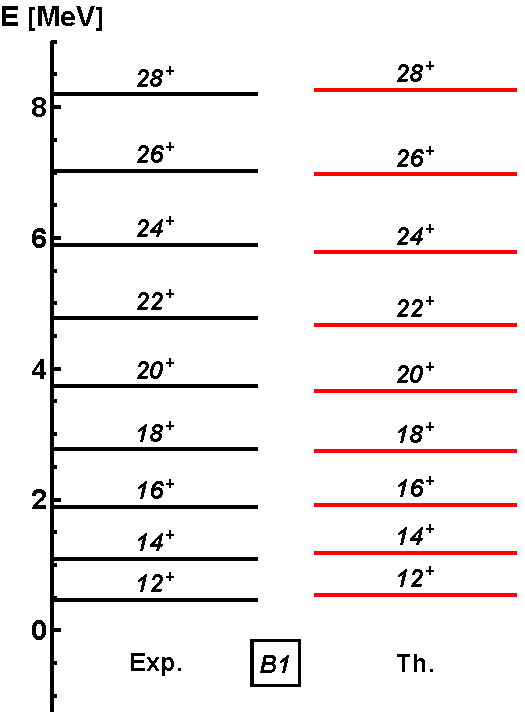
\includegraphics[width=0.46\textwidth]{Chapters/Figures/ba130-band1.pdf}
    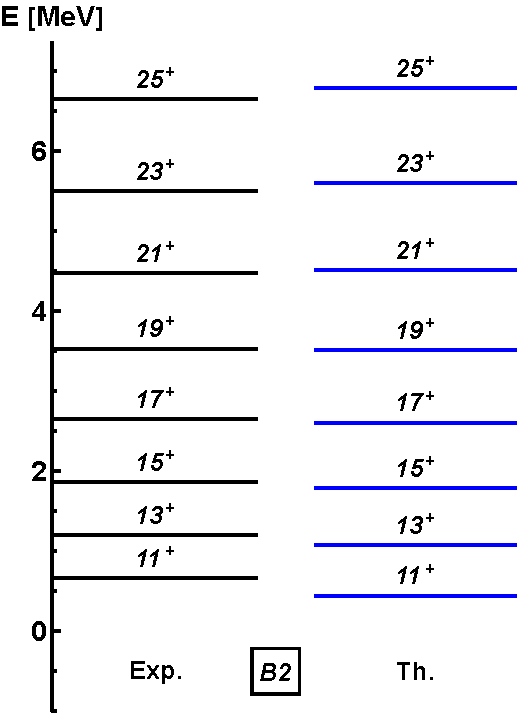
\includegraphics[width=0.46\textwidth]{Chapters/Figures/ba130-band2.pdf}
    \caption{Comparison between the experimental and theoretical excitation energies (Eq. \ref{excitation-energy-general-formula}) for the two wobbling bands of $^{130}$Ba (B1 and B2). Experimental data are taken from Ref. \cite{petrache2019diversity}. The theoretical data was obtained by fitting Eq. \ref{eq-wobbling-energy-evenA} as described in text, with the parameters defined in Table \ref{table-params-ba130}. Note that the band-head $I^\pi=10^+$ state from B1 is missing from the spectrum, since it was subtracted from each level.}
    \label{plot-ba130-excitation-energies}
\end{figure}

Besides the excited spectrum obtained in Fig. \ref{plot-ba130-excitation-energies}, other quantities such as the rotational frequencies for the two bands in $^{130}$Ba are compared with experimental values in Fig. \ref{wobbling-energies-130ba-expVSth}, and the obtained results agree with the measured data quite well. Note that both frequencies are increasing functions of angular momentum, although for B1, at spin $I\geq 24\hbar$, there seems to be a less of an increase, which is not fully reproduced by the fitted values. Moreover, having the excitation energies for the two bands, one can evaluate the theoretical wobbling energies as defined in Eq. \ref{eq-wobbling-energy-definition-evenA} and compare them with the experimental values. The two quantities are graphically represented in Fig. \ref{wobbling-energies-130ba-expVSth}. Remarking the fact that there is an opposite behavior for the two curves, namely the experimental wobbling energies decrease with angular momentum, while the theoretical ones are constantly increasing. Unfortunately, it turns out that by using the Hamiltonian for a \emph{simple wobbler} is not enough to completely describe the collective motion in this isotope.

\begin{figure}
    \centering
    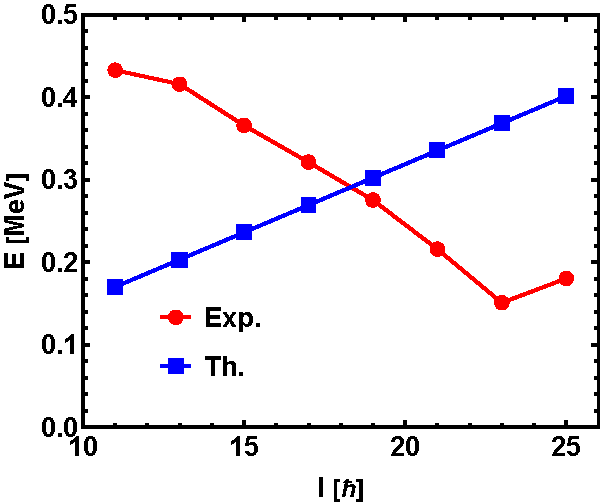
\includegraphics[scale=0.73]{Chapters/Figures/ba130-wobbling-energies.pdf}
    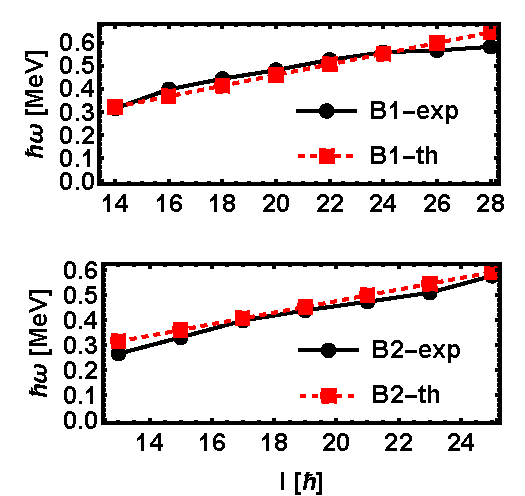
\includegraphics[scale=0.7]{Chapters/Figures/ba130-rotational-frequencies.pdf}
    \caption{\textbf{Left:} The wobbling energies for $^{130}$Ba calculated with Eq. \ref{eq-wobbling-energy-definition-evenA}. For the first state of B2, the energy was determined as $E_\text{wob}(11^+)=E_\text{B2}(11^+)-\frac{1}{2}E_\text{B1}(12^+)$ since the band-head state of B1 is zero (as per the definition of excitation energy given in Eq. \ref{excitation-energy-general-formula}). \textbf{Right:} The rotational frequencies for the two wobbling bands of $^{130}$Ba, calculated using Eq. \ref{rotational-frequency-canonical}.}
    \label{wobbling-energies-130ba-expVSth}
\end{figure}

\subsubsection{Transition Probabilities}

Another step regarding the calculations for $^{130}$Ba consists of the electromagnetic transition probabilities. For this investigation some prior quantities are required. Firstly, the reduced transition probabilities $B(E2)$ (both the interband and the intraband) depend on the components $Q_{20}$ and $Q_{22}$ of the quadrupole moment. These two can be evaluated numerically using the expressions from Eq. \ref{quadrupole-components-q20-q22}, while the intrinsic quadrupole moment is furthermore evaluated using Eq. \ref{quadrupole-moment-Q0}. From the microscopic calculations performed by Chen et al. in Ref. \cite{chen2019transverse}, they determined that this isotope has a stable triaxial minimum located at $(\beta_2,\gamma)=(0.24,21.5^\circ)$. Within the following computations, this set of deformation parameters will be used. Taking the value of $\beta_2=0.24$, the intrinsic quadrupole moment $Q_0$ is readily obtained from Eq. \ref{quadrupole-moment-Q0}. The transition probabilities from Eqs. \ref{intraband-probability-simple-wobbler}, \ref{interband-probability-simple-wobbler-1}, and \ref{interband-probability-simple-wobbler-2} also depend on the two factors $w_{1,2}$ defined in Eq. \ref{eqs-w1-w2-terms-wobbling}, which are functions of the three moments of inertia. Thus, the quality of the fitting procedure will also reflect the calculus for the transition probabilities through $\mathcal{P}_\text{fit}$. The numerical values for $Q_0$, $w_{1,2}$, and $Q_{20,22}$ are presented in Table \ref{transition-parameters-ba130}. Having the deformation parameters, the $w_{1,2}$ terms, and the quadrupole components, one can evaluate the reduced transition probabilities. 

\begin{table}
    \centering
    \begin{tabular}{|c|c|c|}
    % \begin{tabular}{|p{0.15\linewidth}|p{0.25\linewidth}|p{0.5\linewidth}|}
    \hline
    Parameters & Calculated values & Observations                                               \\ \hline
    $\beta_2$  & 0.24              & Taken from Ref. \cite{chen2019transverse}                 \\ \hline
    $\gamma$   & $21.4^\circ$      & Taken from Ref. \cite{chen2019transverse}                 \\ \hline
    $w_1$      & 1.008             & Evaluated with $\mathcal{P}_\text{fit}$                    \\ \hline
    $w_2$      & 0.132             & Evaluated with $\mathcal{P}_\text{fit}$                    \\ \hline
    $Q_0$      & 390.376 $eb\cdot10^{-2}$      & As per Eq. \ref{quadrupole-moment-Q0}                                                           \\ \hline
    $Q_{20}$   & 363.213 $eb\cdot10^{-2}$          & As per Eq. \ref{quadrupole-components-q20-q22}                                                            \\ \hline
    $Q_{22}$   & 101.168 $eb\cdot10^{-2}$           & As per Eq. \ref{quadrupole-components-q20-q22}                                                            \\ \hline
    $B(E2)_\text{in}$ &        0.0509 $(eb)^2$          & Eq. \ref{intraband-probability-simple-wobbler}              \\ \hline
    \end{tabular}%
    \caption{The numerical values for the quantities which are required to determine the quadrupole transition probabilities $B(E2)$ defined in Eqs. \ref{intraband-probability-simple-wobbler} - \ref{interband-probability-simple-wobbler-2}. The parameter set $\mathcal{P}_\text{fit}$ was obtained through the fitting procedure and the values are shown in Table \ref{table-params-ba130}. The intraband transition probabilities $B(E2)$ are evaluated for states $(n,I)\to(,,I-2)$.}
    \label{transition-parameters-ba130}
\end{table}

The graphical representation from Fig. \ref{BE2out-transitions-130ba} shows the interband transition probabilities $B(E2)_\text{out}$ for states $(n_w=1,I)\to(n_w=0,I-1)$. These values are determined with the parameters defined in Table \ref{transition-parameters-ba130}. A constant decrease with spin can be observed, and an overall agreement with theoretical calculations from Ref. \cite{chen2019transverse} is observed (see inset $a$ from Fig. 4).

\begin{figure}
    \centering
    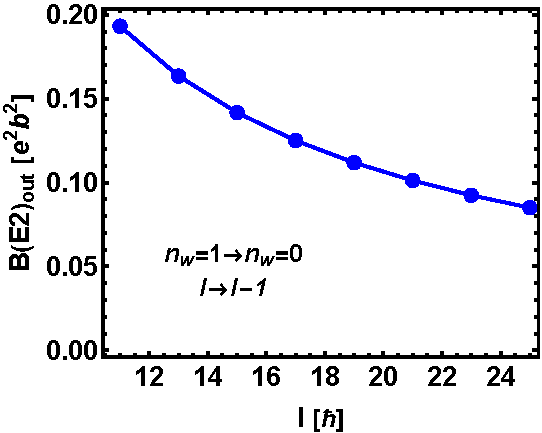
\includegraphics[scale=0.7]{Chapters/Figures/BE2-out-130Ba.pdf}
    \caption{The interband quadrupole transition probabilities (Eq. \ref{interband-probability-simple-wobbler-1}) from the first excited wobbling band (B2) to the yrast band (B1) for $^{130}$Ba.}
    \label{BE2out-transitions-130ba}
\end{figure}

Considering the interband transitions $B(E2)_\text{out}$ calculated above and the constant value for $B(E2)_\text{in}$ (typical for the HA), the ratios $B(E2)_\text{out}/B(E2)_\text{in}$ can also be evaluated. These values are good indicators if a nucleus has a strong deformation and for a wobbler, they lie within $0.2-0.5$. In Table \ref{BE2-out-in-ratio-130Ba}, the obtained ratios are compared with the experimental ones, where a decent agreement can be seen. The theoretical values are decreasing with spin.

\begin{table}
    \centering
    \begin{tabular}{|c|cc|}
    \hline
    \multirow{2}{*}{$I$} & \multicolumn{2}{c|}{$\frac{B(E2)_\text{out}}{B(E2)_\text{in}}$} \\ \cline{2-3} 
                         & \multicolumn{1}{c|}{Experimental}          & Calculated         \\ \hline
    11                   & \multicolumn{1}{c|}{}                      & 0.37           \\ \hline
    13                   & \multicolumn{1}{c|}{0.32}                  & 0.32           \\ \hline
    15                   & \multicolumn{1}{c|}{0.36}                  & 0.27           \\ \hline
    17                   & \multicolumn{1}{c|}{0.22}                  & 0.24           \\ \hline
    19                   & \multicolumn{1}{c|}{0.22}                  & 0.21           \\ \hline
    21                   & \multicolumn{1}{c|}{0.41}                  & 0.19           \\ \hline
    23                   & \multicolumn{1}{c|}{}                      & 0.18           \\ \hline
    25                   & \multicolumn{1}{c|}{}                      & 0.16           \\ \hline
    \end{tabular}%
    \caption{The ratios $\frac{B(E2)_\text{out}}{B(E2)_\text{in}}$ for $^{130}$Ba. The interband transitions signify the change from a state $I$ in B2 to a state $I-1$ in B1. The experimental data (where available) was taken from Ref. \cite{petrache2019diversity,chen2019transverse}.}
    \label{BE2-out-in-ratio-130Ba}
\end{table}

\subsubsection{General Discussion}

Even though the spectrum of this even-even nucleus has been quantitatively reproduced quite well and the values for the tree obtained MOI indicate a triaxial nucleus with main rotation around the third axis, it should not be considered a `realistic' tool in describing this isotope. This is because in another work, Chen et al. \cite{chen2019transverse} found through microscopic calculations that the wobbling motion does not occur as per a pure triaxial rotator, but it emerges from the coupling of two quasi-particles $\pi(h_{11/2})^2$ with a triaxial core. In fact, their work shows that $^{130}$Ba is the first nucleus in which a configuration with two quasi-particles generates stable triaxial deformation through wobbling motion. Consequently, the numerical implementation performed here only shows that HA can be a suitable tool to show that $^{130}$Ba does behave as a wobbler, but this pure triaxial rotator model \emph{hides} contributions coming from single-particle configuration within the final Hamiltonian. This translates to the fact that Eq. \ref{eq-wobbling-energy-evenA} contains the effect of the two $h_{11/2}$ protons hidden within $\hbar\omega_w$. In fact, looking back at $E_\text{wob}$ from Fig. \ref{wobbling-energies-130ba-expVSth}, the discrepancy of the two lines is a clear indicator that some other terms should be taken into account. Also, it is worth mentioning that a quenching factor was necessary in the expression of $B(E2)_\text{in,out}$ in order to compensate for the magnitude of $w_{1,2}$. Nevertheless, this simple and straightforward formalism used to describe the wobbling bands in the even-even $^{130}$Ba nucleus proves to be a decent tool. The calculations presented here have been done independently by the current team, and the obtained results are unique to this research. They will be considered towards a separate forthcoming publication.

Concluding this section on wobbling motion of even-even nuclei, a final sketch is depicted in Fig. \ref{simple-wobbler-geometrical-schematic}, where the main axes of the triaxial ellipsoid are represented and denoted with $m$, $s$, and $l$-axis (medium, short and long, respectively). The precession motion of the total angular momentum (the a.m. of the core itself) will be around the $m$-axis, having the largest moment of inertia.

\begin{figure}
    \centering
    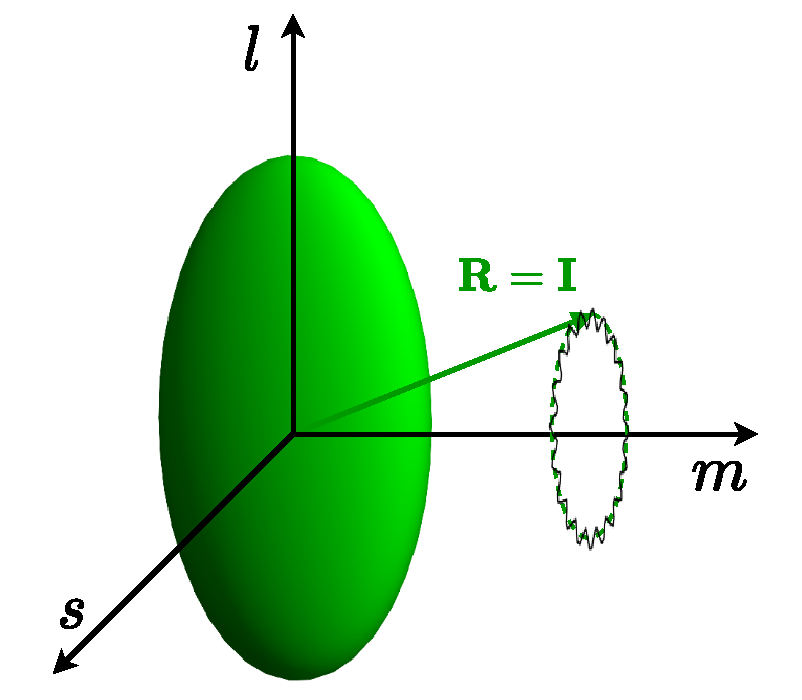
\includegraphics[scale=0.6]{Chapters/Figures/simple_wobbler-schematic.pdf}
    \caption{A schematic representation with a \emph{simple wobbler}, with the total angular momentum doing a precessional motion about the axis with the largest MOI. In this particular sketch, the axis with the largest MOI is denoted with $m$ for intermediate/medium. The $l$- and $s$-axis represent the long and short axes, respectively. The small-amplitude oscillations of $\mathbf{R}_\mathscr{C}$ are depicted with the (black) encircled sine wave. This figure was adapted from Ref. \cite{poenaru2021extensive1} and inspired from Ref. \cite{sensharma2020longitudinal}.}
    \label{simple-wobbler-geometrical-schematic}
\end{figure}

\section{Wobbling Motion in Odd-Mass Nuclei}

The previous discussion regarding the \emph{simple wobbler} was specific to nuclei with even number of nucleons. However, wobbling motion does also occur in odd-mass isotopes. In fact, it turns out that across the chart of nuclides, most of the wobblers are odd-$A$. The reason for this has to do with the triaxial nature of a nucleus. In simple terms, it is `easier' for a (non-axial) deformed system to achieve stability if there is a valence nucleon in a high-$j$ shell which couples to a triaxial core and then drives the entire system to large deformation (remember that different nucleon orbitals will favor specific $\gamma$ values for reaching stable minima).

As an example, for nuclei in the region $N\approx 94$, stable triaxial shapes with large deformations emerge (e.g., $\beta_2\approx0.4$.). These are built on the configuration in which an odd nucleon (i.e., the $i_{13/2}$ proton) couples to a triaxial even-even core. This highly aligned proton will play a crucial role in generating the wobbling excitations for these nuclei by driving the nuclear shape towards large deformations and stabilizing the TSD shapes. Based on this, the description for wobbling motion in an odd-mass system will require the usage of a typical Particle-Rotor-Model that was previously discussed. More precisely, since the core can couple with a particle or hole, and since the deformed system is triaxial, then a particle + rotor model is needed \cite{frauendorf2014transverse}. The model Hamiltonian can be expressed as:
\begin{align}
    \hat{H}=H_\text{coupl.}+\sum_{k=1}^{3}A_k(\hat{I}_k-\hat{j}_k)^2\ ,
    \label{oddA-QTR-general-hamiltonian}
\end{align}
where the odd quasi-particle's a.m. is denoted by $\hat{j}$ and the total a.m. is denoted by $\hat{I}_k$. $H_\text{coupl.}$ defines the coupling of the odd nucleon with the triaxial core. This model is known as \emph{Quasi-Particle Triaxial Rotor} (QTR) and it has been properly developed by Frauendorf et al. in Ref. \cite{frauendorf2014transverse}. Therein, the description for the collective motion in odd-mass nuclei consists in the special distinction between two types of wobbling motion, namely the \emph{longitudinal wobbling motion} and the \emph{transverse wobbling motion}. These two scenarios are dictated by the alignment of the quasi-particle with the axis with the largest MOI of the triaxial ellipsoid. The core + quasi-particle system is regarded as a valence nucleon moving in a quadrupole deformed mea-field generated by the core, so the coupling term $H_\text{coupl.}$ can be considered as the single-particle term presented in Eqs. \ref{single-particle-energies-hpn} and \ref{single-particle-nilsson-defored-potential}.

In the following discussion, some notations will be employed, in order to avoid repeating certain words. Namely, a quasi-particle $\mathcal{Q}$ with hole character will be referred to as $\mathcal{Q}_h$, a proton/neutron will be labelled as $\mathcal{Q}_p$, and the core will be denoted with $\mathscr{C}$. These notations can be seen in Table \ref{notation-table-wobbling}.
\begin{table}
    \centering
    \resizebox{0.8\textwidth}{!}{%
    \begin{tabular}{|c|c|c|}
    \hline
    Object                                                       & Notation                    & Angular momentum             \\ \hline
    quasi-particle                                                 & $\mathcal{Q}$               & $\mathbf{j}_{\mathcal{Q}}$   \\ \hline
    q-p with \emph{particle} character & $\mathcal{Q}_p$             & $\mathbf{j}_{\mathcal{Q}_p}$ \\ \hline
    q-p with \emph{hole} character     & $\mathcal{Q}_h$             & $\mathbf{j}_{\mathcal{Q}_h}$ \\ \hline
    triaxial even-even core                                        & $\mathscr{C}$               & $\mathbf{R}_\mathscr{C}$    \\ \hline
    total system                        & $(\mathcal{Q}+\mathscr{C})$ & $\mathbf{I}$                             \\ \hline
    \end{tabular}%
    }
    \caption{The notations used within the section which describe the QTR, typical for odd-$A$ nuclei.}
    \label{notation-table-wobbling}
\end{table}

The stability of the triaxial nuclear shapes consists of existence of minima within the energy function (see discussion on PES given in Section \ref{potential-energy-surfaces-section}). In order to minimize the system's energy, a $\mathcal{Q}_p$ ($\mathcal{Q}_h$) will tend to create a specific coupling with $\mathscr{C}$, such that their density distribution overlap become maximal (minimal). A maximal (minimal) overlap for $\mathcal{Q}_p+\mathscr{C}$ ($\mathcal{Q}_h+\mathscr{C}$) will minimize the attractive (repulsive) short-range interaction between the two. In terms of the coupling, one can have \cite{frauendorf2014transverse}:
\begin{itemize}
    \item the angular momentum for a high-$j$ $\mathcal{Q}_p$ will align itself with the short $s$-axis of $\mathscr{C}$ 
    \item the angular momentum for a high-$j$ $\mathcal{Q}_h$ will align itself with the long $l$-axis of $\mathscr{C}$
    \item the angular momentum for any $\mathcal{Q}$ from a half-filled high-$j$ shell will align itself with the intermediate $m$-axis of $\mathscr{C}$
\end{itemize}
Going back to the two wobbling modes for an odd-$A$ nucleus, the $\mathcal{Q}+\mathscr{C}$ coupling dictates which one of the wobbling modes will arise. More precisely, if the a.m. for $\mathcal{Q}$ aligns itself \emph{along} the $m$-axis, then the motion is considered \emph{longitudinal wobbling} (LW). On the other hand, if the a.m. for $\mathcal{Q}$ aligns itself \emph{perpendicular} to the $m$-axis, then the motion is considered as \emph{transverse wobbling} (TW). One can encounter two different situations that could lead to transverse wobbling. If a $\mathcal{Q}_p$ comes from the bottom of a deformed $j$-shell, it will align its a.m. with the $s$-axis (i.e., $s\perp m$). Moreover, if a $\mathcal{Q}_h$ comes from the top of a deformed $j$-shell, it will tend to align its a.m. with the $l$-axis (see discussion in Section \ref{chiral-section}). These three scenarios are summarized in three \emph{workflow diagrams} that aim to depict the wobbling motion (stable triaxial structures), starting from the quasi-particle position within a $j$-shell and ending with the emerging wobbling behavior. For the TW case, one can see the sketches from Figs. \ref{advanced-quasiparticle-coupling-1}-\ref{advanced-quasiparticle-coupling-2}, while the same analogy is shown in Fig. \ref{advanced-quasiparticle-coupling-3} for LW.
\begin{figure}
    \centering
    \begin{tikzpicture}[every text node part/.style={align=center}]
        % draw a background box for the density overlap and the two gaussian curves
        \node[rectangle, very thick,dashed,draw=black,fill=none] (huge-container-box) [minimum height=5cm,minimum width=12cm,xshift=0.7cm,yshift=-0.3cm] at (2,2.5) {};
        \begin{scope}[xshift=1cm]
            % add coupling schematic
            \draw[-latex] [thick, color=black,dashed] (1.5,6) -- (6,6) node [yshift=-0.3cm] {$m$-axis};
            \draw[-latex] [ultra thick, color=black,dashed] (1.5,6) -- (6,6) node [yshift=+0.4cm,xshift=0.3cm] {$\mathcal{I}_m>(\mathcal{I}_{l},\mathcal{I}_{s})$};
            \draw[-latex] [thick, color=black,dashed] (1.5,6) -- (1.5,9) node [pos=1,above] {$s$-axis};
            \draw[-latex] [ultra thick, color=black!60!green] (1.5,6) -- (4,6.6) node [yshift=0.3cm,xshift=-0.5cm] {$\mathbf{R}_{\mathscr{C}}$};
            \draw[-latex] [ultra thick, color=magenta] (1.5,6) -- (1.5,8) node [xshift=-0.5cm] (my-arrow) {$\mathbf{j}_{\mathcal{Q}_p}$};
            % \draw[-latex] [ultra thick, color=magenta] (1.5,6) -- (1.5,8) node [pos=1,above,xshift=-1cm] (my-arrow) {$\mathbf{j}_{\mathcal{Q}_p}$};
            \node[rectangle, draw=black, fill=none,anchor=south west] at (1.5,6) {};
            \node[rectangle, draw=black, fill=green!10,anchor=south west, minimum width=4cm] at (3,7.5) (coupling-box) {$(\mathcal{Q}_p+\mathscr{C})$\\ Coupling};
        \end{scope}
        
        \node[rectangle, draw=black, thick, fill=green!10, inner sep=0.2cm,minimum width=8 cm] at (2,-1.8) (first-box) {\textbf{Minimized} short-range interaction \\ \\ $\mathcal{Q}_p+\mathscr{C}$ = \emph{attractive}};
        \node[rectangle] (pes-image-box) [right=of first-box,xshift=-0.7cm] {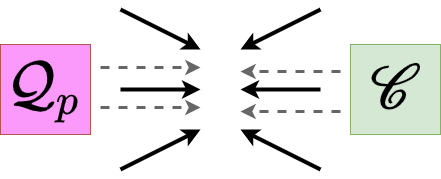
\includegraphics[scale=0.2]{Chapters/Figures/attractive_interaction.png}};
        
        \node[rectangle, draw=black, thick, fill=green!10, inner sep=0.2cm,minimum width=8 cm] (second-box) [below=of first-box] {\textbf{Minimal} energy (PES)};
        \node[rectangle] (pes-image-box) [right=of second-box,xshift=-0.7cm,yshift=0.4cm] {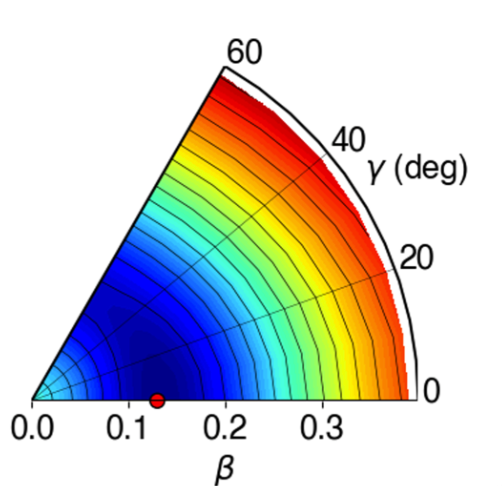
\includegraphics[scale=0.12]{Chapters/Figures/PES_small_update.png}};
        
        \node[rectangle, draw=black, thick, fill=green!10, inner sep=0.2cm,minimum width=8 cm] (third-box) [below=of second-box] {\textbf{Stable triaxial shape} \\ $\downarrow$ \\ \textbf{Transverse Wobbling Motion}: \\ $\mathbf{j}_{\mathcal{Q}_p}\perp \mathbf{m}_\text{axis}$};
        \node[rectangle] (precession-cone-box) [right=of third-box,xshift=-1cm] {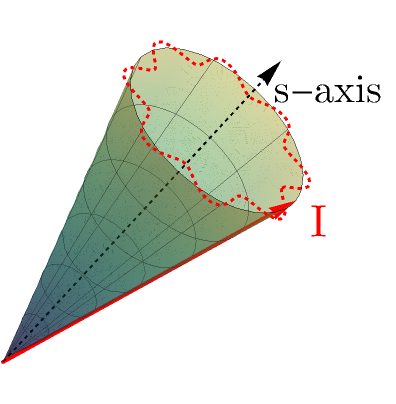
\includegraphics[scale=0.3]{Chapters/Figures/precessional_cone.png}};
        
        \node[rectangle, draw=black,xshift=6cm,yshift=2cm,fill=green!10, minimum width=4cm] (maximal-box) {\textbf{Maximal overlap} \\ between \\ {\color{magenta}$\mathcal{D}\left(\mathcal{Q}_p\right)$} and {\color{black!60!green}$\mathcal{D}\left(\mathscr{C}\right)$}};


        % \draw[-latex] [very thick,black] (inside-node.east) -- ($(inside-node.east)+(2.2,0)$) |- node [xshift=-1.9cm,yshift=2.7cm] (maximal-box) {\textbf{Maximal overlap} \\ between \\ {\color{magenta}$\mathcal{D}\left(\mathcal{Q}_p\right)$} and {\color{black!60!green}$\mathcal{D}\left(\mathscr{C}\right)$}} (first-box.east);
        % \draw[-latex] [very thick,black] (first-box) -- node[circle,draw=black,xshift=1cm] {a} (second-box);
        \draw[-latex] [very thick,black] (first-box) -- node[circle,draw=black,xshift=1cm,fill=yellow!30] {$4$} (second-box);
        \draw[-latex] [very thick,black] (second-box) -- node[circle,draw=black,xshift=1cm,fill=yellow!30] {$5$} (third-box);
        % \draw[-latex] [very thick, color=black] (1.5,5.5) -| (maximal-box.east);
        
        % draw arrow for coupling and maximal overlap
        \draw[-latex] [very thick, color=black] (coupling-box.east) -- ($(coupling-box.east)+(1,0)$) |- node[circle,draw=black,xshift=-0.4cm,yshift=-0.6cm,fill=yellow!30] {$2$} (maximal-box.east);

        \begin{axis}[scale=0.6,xshift=-2cm,every axis plot post/.append style={
            mark=none,domain=-2:3,samples=50,smooth}, % All plots: from -2:2, 50 samples, smooth, no marks
            axis x line*=bottom, % no box around the plot, only x and y axis
            axis y line*=left, % the * suppresses the arrow tips
            axis line style={draw=none},
            xtick=\empty, ytick=\empty,
            enlargelimits=false, 
            clip=false, 
            axis on top,
            grid = major,
            legend style={at={(1,1)},anchor=north,legend cell align=left}
            ]
            % extend the axes a bit to the right and top
            
            \addplot [name path=particle-density, color=magenta,ultra thick] {\gauss{0}{0.5}};
            \addplot [name path=core-density, color=black!60!green,ultra thick] {\gauss{0.4}{0.7}};
            \legend{$\mathcal{D}\left(\mathcal{Q}_p\right)$,$\mathcal{D}\left(\mathscr{C}\right)$}
            \path[name path=axis] (axis cs:1,0) -- (axis cs:2,0);
            
            % path for fixing boundaries which will be used to fill common region between gaussian curves
            \path[name path=lower,intersection segments={of=particle-density and core-density, sequence={L1 -- R2 -- L3}}];
            
            \node[rectangle, draw=none, thick, fill=none] at (axis cs: 0.8,0.9) (inside-node) {Density distributions for $\mathcal{Q}_p$ and $\mathscr{C}$};
            
            \addplot[color=gray!30] fill between[of= lower and axis];
        \end{axis}

        \begin{scope}[yshift=6cm,xshift=-4cm]
            % draw Fermi orbital for a j-particle
            \node[rectangle, very thick,draw=black,fill=yellow!50] (jshell-box) [minimum height=3cm,minimum width=2cm] at (2.5,1.5) {};
            \foreach \x [count=\xi] in {0.1,0.2,0.3,0.4,0.5,0.6} { 
                \draw (2,\xi em) -- (3,\xi em) ;
            }
            \node at (1.8,0.4) {$\mathcal{Q}_p$};
            \node[circle,draw=none,fill=magenta] at (2.5,0.4) {};
            \node[] at (2.5,-0.5) {$j$-shell};
        \end{scope}

        %draw arrow from jshell to coupling box
        \draw[-latex,very thick] (jshell-box.north) -- ($(jshell-box.north)+(0,1cm)$) node[circle,draw=black,yshift=-0.6cm,xshift=8.1cm,fill=yellow!30] {$1$} -| (coupling-box);

        % connect maximal overlap with minimal interaction
        \draw[-latex,very thick] (maximal-box.south) -- ($(maximal-box.south)-(0,0.4cm)$) -| node[draw=black,circle,yshift=-0.5cm,xshift=0.6cm,fill=yellow!30] {$3$} ([xshift=1cm]first-box.north);
    \end{tikzpicture}
    \caption{The workflow of a quasi-particle with particle character $\mathcal{Q}_p$ in its coupling with a triaxial rotor $\mathscr{C}$. Each of the five `steps' represents a characteristic involved in the wobbling motion, as described in text. Namely, for $\mathcal{Q}_p$ coming from the bottom of a $j$-shell and coupling with the $s$-axis of the even-even core $\mathscr{C}$ \textbf{(1)} will maximize the density overlap \textbf{(2)}, which will minimize their interaction \textbf{(3)}, minimizing the total energy \textbf{(4)}, and finally stabilizing the triaxial structure \textbf{(5)} to a TW. The long $l$-axis has been ignored within the drawings. In the bottom-most picture, the precessional cone of the total a.m. is shown, oscillating along the $s$-axis.}
    \label{advanced-quasiparticle-coupling-1}
\end{figure}
\begin{figure}
\centering
\begin{tikzpicture}[every text node part/.style={align=center}]
    % draw a background box for the density overlap and the two gaussian curves
    \node[rectangle, very thick,dashed,draw=black,fill=none] (huge-container-box) [minimum height=5cm,minimum width=12cm,xshift=0.7cm,yshift=-0.3cm] at (2,2.5) {};
    \begin{scope}[xshift=1cm]
        % add coupling schematic
        \draw[-latex] [thick, color=black,dashed] (1.5,6) -- (6,6) node [yshift=-0.3cm] {$m$-axis};
        \draw[-latex] [ultra thick, color=black,dashed] (1.5,6) -- (6,6) node [yshift=+0.4cm,xshift=0.3cm] {$\mathcal{I}_m>(\mathcal{I}_{l},\mathcal{I}_{s})$};
        \draw[-latex] [thick, color=black,dashed] (1.5,6) -- (1.5,9) node [pos=1,above] {$l$-axis};
        \draw[-latex] [ultra thick, color=black!60!green] (1.5,6) -- (4,6.6) node [yshift=0.3cm,xshift=-0.5cm] {$\mathbf{R}_{\mathscr{C}}$};
        \draw[-latex] [ultra thick, color=blue] (1.5,6) -- (1.5,8) node [xshift=-0.5cm] (my-arrow) {$\mathbf{j}_{\mathcal{Q}_h}$};
        % \draw[-latex] [ultra thick, color=magenta] (1.5,6) -- (1.5,8) node [pos=1,above,xshift=-1cm] (my-arrow) {$\mathbf{j}_{\mathcal{Q}_p}$};
        \node[rectangle, draw=black, fill=none,anchor=south west] at (1.5,6) {};
        \node[rectangle, draw=black, fill=red!10,anchor=south west, minimum width=4cm] at (3,7.5) (coupling-box) {$(\mathcal{Q}_h+\mathscr{C})$\\ Coupling};
    \end{scope}
    
    \node[rectangle, draw=black, thick, fill=red!10, inner sep=0.2cm,minimum width=8 cm] at (2,-1.8) (first-box) {\textbf{Minimized} short-range interaction \\ \\ $(\mathcal{Q}_h+\mathscr{C})$ = \emph{repulsive}};
    \node[rectangle] (pes-image-box) [right=of first-box,xshift=-0.7cm] {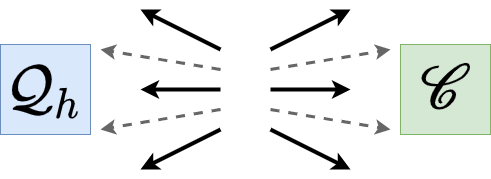
\includegraphics[scale=0.2]{Chapters/Figures/repulsive_interaction.png}};
    
    \node[rectangle, draw=black, thick, fill=red!10, inner sep=0.2cm,minimum width=8 cm] (second-box) [below=of first-box] {\textbf{Minimal} energy (PES)};
    \node[rectangle] (pes-image-box) [right=of second-box,xshift=-0.7cm,yshift=0.4cm] {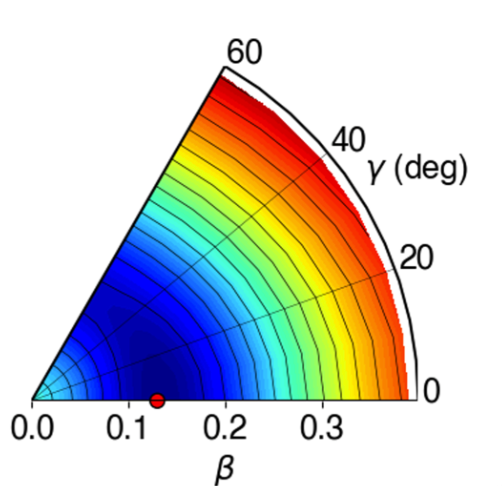
\includegraphics[scale=0.12]{Chapters/Figures/PES_small_update.png}};
    
    \node[rectangle, draw=black, thick, fill=red!10, inner sep=0.2cm,minimum width=8 cm] (third-box) [below=of second-box] {\textbf{Stable triaxial shape} \\ $\downarrow$ \\ \textbf{Transverse Wobbling Motion}: \\ $\mathbf{j}_{\mathcal{Q}_h}\perp \mathbf{m}_\text{axis}$};
    \node[rectangle] (precession-cone-box) [right=of third-box,xshift=-1cm] {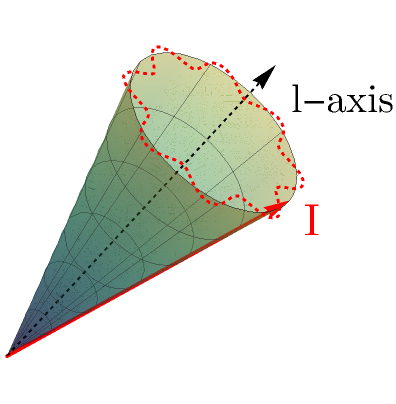
\includegraphics[scale=0.3]{Chapters/Figures/precessional_cone_2.png}};
    
    \node[rectangle, draw=black,xshift=6cm,yshift=2cm,fill=red!10, minimum width=4cm] (maximal-box) {\textbf{Minimal overlap} \\ between \\ {\color{blue}$\mathcal{D}\left(\mathcal{Q}_h\right)$} and {\color{black!60!green}$\mathcal{D}\left(\mathscr{C}\right)$}};


    % \draw[-latex] [very thick,black] (inside-node.east) -- ($(inside-node.east)+(2.2,0)$) |- node [xshift=-1.9cm,yshift=2.7cm] (maximal-box) {\textbf{Maximal overlap} \\ between \\ {\color{magenta}$\mathcal{D}\left(\mathcal{Q}_p\right)$} and {\color{black!60!green}$\mathcal{D}\left(\mathscr{C}\right)$}} (first-box.east);
    % \draw[-latex] [very thick,black] (first-box) -- node[circle,draw=black,xshift=1cm] {a} (second-box);
    \draw[-latex] [very thick,black] (first-box) -- node[circle,draw=black,xshift=1cm,fill=yellow!30] {$4$} (second-box);
    \draw[-latex] [very thick,black] (second-box) -- node[circle,draw=black,xshift=1cm,fill=yellow!30] {$5$} (third-box);
    % \draw[-latex] [very thick, color=black] (1.5,5.5) -| (maximal-box.east);
    
    % draw arrow for coupling and maximal overlap
    \draw[-latex] [very thick, color=black] (coupling-box.east) -- ($(coupling-box.east)+(1,0)$) |- node[circle,draw=black,xshift=-0.4cm,yshift=-0.6cm,fill=yellow!30] {$2$} (maximal-box.east);

    \begin{axis}[scale=0.6,xshift=-2cm,every axis plot post/.append style={
        mark=none,
        domain=0:10,
        samples=50,
        smooth}, % All plots: from -3:3, 50 samples, smooth, no marks
        axis x line*=bottom, % no box around the plot, only x and y axis
        axis y line*=left, % the * suppresses the arrow tips
        axis line style={draw=none},
        xtick=\empty, ytick=\empty,
        enlargelimits=false, 
        clip=false, 
        grid = major,
        legend style={at={(1,1)},anchor=north,legend cell align=left}
        ]
        % extend the axes a bit to the right and top
        
        % \addplot [name path=particle-density, color=blue,very thick] {\gauss{5}{0.4}};
        % \addplot [name path=core-density, color=black!60!green,very thick] {\gauss{5}{0.65}};
        
        % use filling implementation from this pose 
        % source: https://tex.stackexchange.com/a/305677/139074

        \addplot [name path=model,ultra thick, smooth, color=blue] {\gauss{3}{1}};
        \addplot [name path=obs,ultra thick, smooth, color=black!60!green] {\gauss{6.5}{1.2}};
        \legend{$\mathcal{D}\left(\mathcal{Q}_h\right)$,$\mathcal{D}\left(\mathscr{C}\right)$}
        
        \node[rectangle, draw=none, thick, fill=none] at (axis cs: 5.3,0.48) (inside-node) {Density distributions for $\mathcal{Q}_n$ and $\mathscr{C}$};

        \path[name path=lower,
        intersection segments={
        of=model and obs,
        sequence=A0 -- B1}];

        \path[name path=axis] (axis cs:0,0) -- (axis cs:16,0);

        \addplot[color=gray!30]
        fill between[
        of= model and axis]
        ;
        \addplot[color=white]
        fill between[
        of=model and obs,
        soft clip={domain=0:10}]
        ;

    \end{axis}

    \begin{scope}[yshift=6cm,xshift=-4cm]
        % draw Fermi orbital for a j-particle
        \node[rectangle, very thick,draw=black,fill=yellow!50] (jshell-box) [minimum height=3cm,minimum width=2cm] at (2.5,1.5) {};
        \foreach \x [count=\xi] in {0.1,0.2,0.3,0.4,0.5,0.6} { 
            \draw (2,\xi em) -- (3,\xi em) ;
        }
        \node at (1.8,2.5) {$\mathcal{Q}_h$};
        \node[circle,draw=none,fill=blue] at (2.5,2.5) {};
        \node[] at (2.5,-0.5) {$j$-shell};
    \end{scope}

    %draw arrow from jshell to coupling box
    \draw[-latex,very thick] (jshell-box.north) -- ($(jshell-box.north)+(0,1cm)$) node[circle,draw=black,yshift=-0.6cm,xshift=8.1cm,fill=yellow!30] {$1$} -| (coupling-box);

    % connect maximal overlap with minimal interaction
    \draw[-latex,very thick] (maximal-box.south) -- ($(maximal-box.south)-(0,0.4cm)$) -| node[draw=black,circle,yshift=-0.5cm,xshift=0.6cm,fill=yellow!30] {$3$} ([xshift=1cm]first-box.north);
\end{tikzpicture}
\caption{The workflow of a quasi-particle with hole character $\mathcal{Q}_h$ in its coupling with a triaxial rotor $\mathscr{C}$. Each of the five `steps' represents a characteristic involved in the wobbling motion, as described in text. Namely, for $\mathcal{Q}_h$ coming from the top of a $j$-shell and coupling with the $l$-axis of the even-even core $\mathscr{C}$ \textbf{(1)} will minimize the density overlap \textbf{(2)}, which will minimize their interaction \textbf{(3)}, minimizing the total energy \textbf{(4)}, and finally stabilizing the triaxial structure \textbf{(5)} to a TW. The short $s$-axis has been ignored within the drawings. In the bottom-most picture, the precessional cone of the total a.m. is shown, oscillating along the $l$-axis.}
\label{advanced-quasiparticle-coupling-2}
\end{figure}
\begin{figure}
    \centering
    \begin{tikzpicture}[every text node part/.style={align=center}]
        
        % draw a background box for the density overlap and the two gaussian curves
        \node[rectangle, very thick,dashed,draw=black,fill=none] (huge-container-box) [minimum height=5cm,minimum width=12cm,xshift=0.7cm,yshift=-0.3cm] at (2,2.5) {};
        
        \begin{scope}[xshift=1cm]
            % add coupling schematic
            % \draw[-latex] [thick, color=black,dashed] (1.5,6) -- (5.5,6) node [yshift=-0.3cm] {$m$-axis};
            \draw[-latex] [ultra thick, color=black,dashed] (1.5,6) -- (6,6) node [yshift=+0.4cm,xshift=0.3cm] {$\mathcal{I}_m>(\mathcal{I}_{l},\mathcal{I}_{s})$};
            % \draw[-latex] [thick, color=black,dashed] (1.5,6) -- (1.5,9) node [pos=1,above] {$l$-axis};
            \draw[-latex] [ultra thick, color=black!60!green] (1.5,6) -- (4,6.6) node [yshift=0.3cm,xshift=-0.5cm] {$\mathbf{R}_{\mathscr{C}}$};
            \draw[-latex] [ultra thick, color=magenta] (1.5,6) -- (3,6) node [yshift=-0.4cm] (my-arrow) {$\mathbf{j}_{\mathcal{Q}_p}$};
            \node[rectangle, draw=black, fill=blue!10,anchor=south west, minimum width=4cm] at (3,7.5) (coupling-box) {$(\mathcal{Q}_p+\mathscr{C})$\\ Coupling};
        \end{scope}
        
        \node[rectangle, draw=black, thick, fill=blue!10, inner sep=0.2cm,minimum width=8 cm] at (2,-1.8) (first-box) {\textbf{Minimized} short-range interaction \\ \\ $(\mathcal{Q}_p+\mathscr{C})$ = \emph{attractive}};
        \node[rectangle] (pes-image-box) [right=of first-box,xshift=-0.7cm] {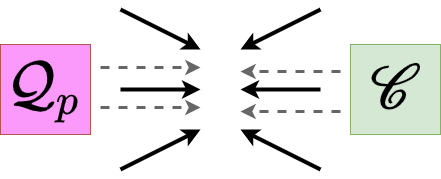
\includegraphics[scale=0.2]{Chapters/Figures/attractive_interaction.png}};
        
        \node[rectangle, draw=black, thick, fill=blue!10, inner sep=0.2cm,minimum width=8 cm] (second-box) [below=of first-box] {\textbf{Minimal} energy (PES)};
        \node[rectangle] (pes-image-box) [right=of second-box,xshift=-0.7cm,yshift=0.4cm] {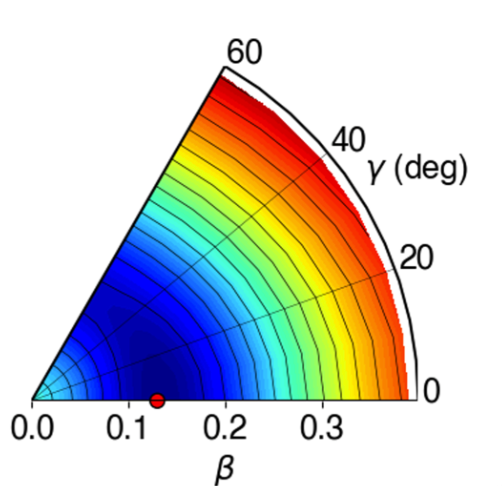
\includegraphics[scale=0.12]{Chapters/Figures/PES_small_update.png}};
        
        \node[rectangle, draw=black, thick, fill=blue!10, inner sep=0.2cm,minimum width=8 cm] (third-box) [below=of second-box] {\textbf{Stable triaxial shape} \\ $\downarrow$ \\ \textbf{Longitudinal Wobbling Motion}: \\ $\mathbf{j}_{\mathcal{Q}_p}\ ||\ \mathbf{m}_\text{axis}$};
        \node[rectangle] (precession-cone-box) [right=of third-box,xshift=-1cm] {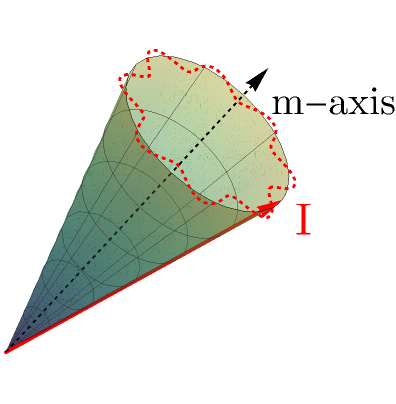
\includegraphics[scale=0.3]{Chapters/Figures/precessional_cone_3.png}};
        
        \node[rectangle, draw=black,xshift=6cm,yshift=2cm,fill=blue!10, minimum width=4cm] (maximal-box) {\textbf{Maximal overlap} \\ between \\ {\color{magenta}$\mathcal{D}\left(\mathcal{Q}_p\right)$} and {\color{black!60!green}$\mathcal{D}\left(\mathscr{C}\right)$}};


        % \draw[-latex] [very thick,black] (inside-node.east) -- ($(inside-node.east)+(2.2,0)$) |- node [xshift=-1.9cm,yshift=2.7cm] (maximal-box) {\textbf{Maximal overlap} \\ between \\ {\color{magenta}$\mathcal{D}\left(\mathcal{Q}_p\right)$} and {\color{black!60!green}$\mathcal{D}\left(\mathscr{C}\right)$}} (first-box.east);
        % \draw[-latex] [very thick,black] (first-box) -- node[circle,draw=black,xshift=1cm] {a} (second-box);
        \draw[-latex] [very thick,black] (first-box) -- node[circle,draw=black,xshift=1cm,fill=yellow!30] {$4$} (second-box);
        \draw[-latex] [very thick,black] (second-box) -- node[circle,draw=black,xshift=1cm,fill=yellow!30] {$5$} (third-box);
        % \draw[-latex] [very thick, color=black] (1.5,5.5) -| (maximal-box.east);
        
        % draw arrow for coupling and maximal overlap
        \draw[-latex] [very thick, color=black] (coupling-box.east) -- ($(coupling-box.east)+(1,0)$) |- node[circle,draw=black,xshift=-0.4cm,yshift=-0.6cm,fill=yellow!30] {$2$} (maximal-box.east);

        \begin{axis}[scale=0.6,xshift=-2cm,every axis plot post/.append style={
            mark=none,
            domain=0:10,
            samples=50,
            smooth}, % All plots: from -3:3, 50 samples, smooth, no marks
            axis x line*=bottom, % no box around the plot, only x and y axis
            axis y line*=left, % the * suppresses the arrow tips
            axis line style={draw=none},
            xtick=\empty, ytick=\empty,
            enlargelimits=false, 
            clip=false, 
            grid = major,
            legend style={at={(1,1)},anchor=north,legend cell align=left}
            ]
            % extend the axes a bit to the right and top
            
            % \addplot [name path=particle-density, color=blue,very thick] {\gauss{5}{0.4}};
            % \addplot [name path=core-density, color=black!60!green,very thick] {\gauss{5}{0.65}};
            
            % use filling implementation from this pose 
            % source: https://tex.stackexchange.com/a/305677/139074

            \addplot [name path=model,ultra thick, smooth, color=magenta] {\gauss{2.8}{1}};
            \addplot [name path=obs,ultra thick, smooth, color=black!60!green] {\gauss{3.5}{1.3}};
            \legend{$\mathcal{D}\left(\mathcal{Q}_p\right)$,$\mathcal{D}\left(\mathscr{C}\right)$}
            
            \node[rectangle, draw=none, thick, fill=none] at (axis cs: 5.3,0.48) (inside-node) {Density distributions for $\mathcal{Q}_p$ and $\mathscr{C}$};


            \path[name path=lower,
            intersection segments={
            of=model and obs,
            sequence=A0 -- B1}];

            \path[name path=axis] (axis cs:0,0) -- (axis cs:16,0);

            \addplot[color=gray!30]
            fill between[
            of= model and axis]
            ;
            \addplot[color=white]
            fill between[
            of=model and obs,
            soft clip={domain=0:10}]
            ;

        \end{axis}

        \begin{scope}[yshift=6cm,xshift=-4cm]
            % draw Fermi orbital for a j-particle
            \node[rectangle, very thick,draw=black,fill=yellow!50] (jshell-box) [minimum height=3cm,minimum width=2cm] at (2.5,1.5) {};
            \foreach \x [count=\xi] in {0.1,0.2,0.3,0.4,0.5,0.6} { 
                \draw (2,\xi em) -- (3,\xi em) ;
            }
            \node at (1.8,1.25) {$\mathcal{Q}_p$};
            \node[circle,draw=none,fill=magenta] at (2.5,1.25) {};
            \node[] at (2.5,-0.5) {$j$-shell};
        \end{scope}

        %draw arrow from jshell to coupling box
        \draw[-latex,very thick] (jshell-box.north) -- ($(jshell-box.north)+(0,1cm)$) node[circle,draw=black,yshift=-0.6cm,xshift=8.1cm,fill=yellow!30] {$1$} -| (coupling-box);

        % connect maximal overlap with minimal interaction
        \draw[-latex,very thick] (maximal-box.south) -- ($(maximal-box.south)-(0,0.4cm)$) -| node[draw=black,circle,yshift=-0.5cm,xshift=0.6cm,fill=yellow!30] {$3$} ([xshift=1cm]first-box.north);
    
    \end{tikzpicture}
    
    \caption{The workflow of a particle $\mathcal{Q}_p$ in its coupling with a triaxial rotor $\mathscr{C}$ within LW mode. Each of the five `steps' represents a characteristic involved in the wobbling motion, as described in text. Namely, for $\mathcal{Q}_p$ coming from the middle of a $j$-shell and coupling with the $m$-axis of the even-even core $\mathscr{C}$ \textbf{(1)} will maximize the density overlap \textbf{(2)}, which will minimize their interaction \textbf{(3)}, minimizing the total energy \textbf{(4)}, and finally stabilizing the triaxial structure \textbf{(5)}. In the bottom-most picture, the precessional cone of the total a.m. is shown, oscillating along the $m$-axis.}
    \label{advanced-quasiparticle-coupling-3}
\end{figure}

For increasing rotating motion, the Coriolis effect kicks in, trying to align the angular momentum of $\mathcal{Q}$ with the axis of rotation (i.e., the $m$-axis), creating thus a change from $(s)\to (m)$-axis for $\mathcal{Q}_p$ and a realignment $(l) \to (m)$-axis for $\mathcal{Q}_h$. The realignment will result in a transition from one wobbling regime to another, meaning that the system will undergo a phase transition. This kind of change can take place at some `critical' value for the nuclear spin $I$. In a recent work made by this team \cite{poenaru2021extensive1,poenaru2021extensive2} such a transition is discussed within a semi-classical approach.

Hamiltonian given in Eq. \ref{oddA-QTR-general-hamiltonian} can be treated in the so-called \emph{Frozen Alignment} (FA) approximation, employed in \cite{frauendorf2014transverse}. The idea behind FA is that the a.m. for $\mathcal{Q}$ is fixed (i.e., rigidly aligned) with one of the principal axes of $\mathscr{C}$. In fact, this rigid coupling is an idealistic situation of either a LW regime or a TW mode. Furthermore, if one applies the small-amplitude limit for wobbling vibrations about the three-axis (i.e., a Harmonic Approximation as the one used for the simple wobbler), then the Hamiltonian will become:
\begin{align}
    \hat{H}=A_3(\hat{I}_3-j)^2+A_1\hat{I}_1^2+A_2\hat{I}_2^2\ .
    \label{hamiltonian-qtr-FA}
\end{align}
Indeed, within QTR Hamiltonian from Eq. \ref{hamiltonian-qtr-FA}, the angular momentum for $\mathcal{Q}$ becomes just a number $j$. The quasi-particle $\mathcal{Q}$ is fixed along the three-axis. Regarding the angular momentum components, these can be re-written as:
\begin{align}
    \hat{I}_3=\sqrt{\mathscr{I}^2-\hat{I}_1^2-\hat{I}_1^2}\approx\mathscr{I}-\frac{1}{2}\left(\frac{\hat{I}_1^2}{\mathscr{I}}+\frac{\hat{I}_2^2}{\mathscr{I}}\right)\ ,
\end{align}
where the `eigenvalue' of $I$ is denoted as $\mathscr{I}=\sqrt{I(I+1)}$. Note that this is in fact a second-order expansion in terms of the square-root function. If the factor $A_3$ is also expressed in terms of $j$ and $\mathscr{I}$ (e.g., introducing a so-called \emph{reduced} inertia parameter) via the relation:
\begin{align}
    \mathscr{A}_3=A_3\left(1-\frac{j}{\mathscr{I}}\right)\ ,
    \label{reduced-inertia-parameter-A3}
\end{align}
then the QTR Hamiltonian achieves the following form:
\begin{align}
    \hat{H}={\color{black}A_3(\mathscr{I}-j)^2}+{\color{black}(A_1-\mathscr{A}_3)\hat{I}_1^2+(A_2-\mathscr{A}_3)\hat{I}_2^2}\ .
    \label{HA-QTR-Hamiltonian}
\end{align}

The reduced inertia parameter $\mathscr{A}_3$ is graphically represented in Fig. \ref{reduced-inertia-A3-figs}, where the evolution with spin $I$ is studied for different values of $A_3$ but fixed $j$ (left inset) and fixed $A_3$ but different $j$ (right inset). Keep in mind that the value of the spin $I$ defines the quantity $\mathscr{I}$ which enters in Eq. \ref{reduced-inertia-parameter-A3}.
\begin{figure}
    \centering
    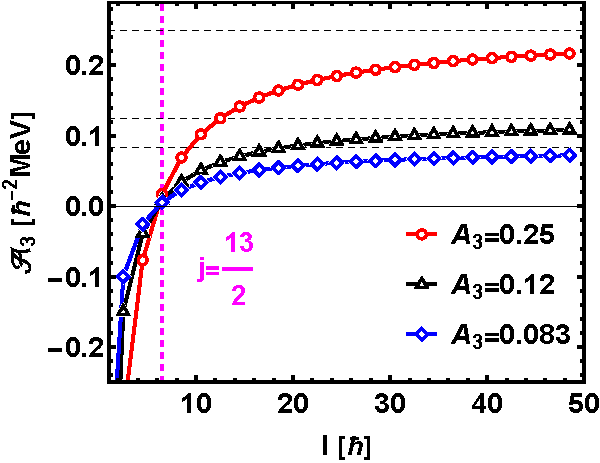
\includegraphics[width=0.49\textwidth]{Chapters/Figures/reducedInertia_fig1.pdf}
    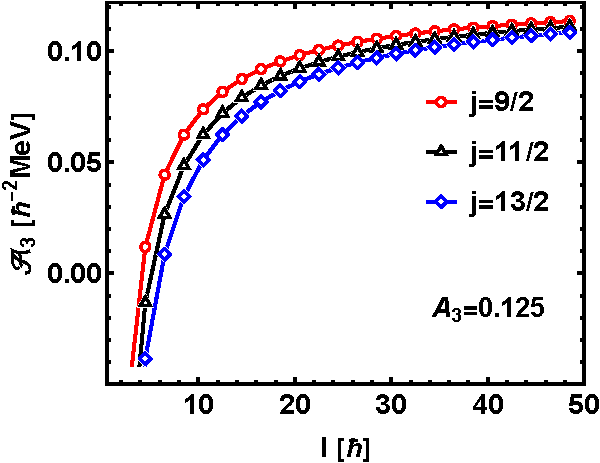
\includegraphics[width=0.49\textwidth]{Chapters/Figures/reducedInertia_fig2.pdf}
    \caption{The reduced inertia parameter defined in Eq. \ref{reduced-inertia-parameter-A3} as a function of spin. \textbf{Left:} The angular momentum of the quasi-particle is fixed (i.e., $j=13/2$) and different values for $A_3$ are attributed. The vertical grid-line corresponds to the value of $j$ at which $\mathscr{A}_3$ becomes positive. The horizontal grid-lines correspond to the numerical values of $A_3$. \textbf{Right:} The value of $A_3$ is fixed and different a.m. values for $j$ are considered. Note that $I$ is used to define $\mathscr{I}$ which appears in the expression of $\mathscr{A}_3$.}
    \label{reduced-inertia-A3-figs}
\end{figure}

The Hamiltonian for an odd-$A$ triaxial nucleus, within the Harmonic Approximation has an expression which at a first glance looks quite similar to the simple wobbler (Eq. \ref{general-rotor-ham-evenA}), except that the coefficients of the first and second components $\hat{I}_{1,2}$ contain a contribution coming from the quasi-particle itself (through the `reduced' inertia parameter $\mathscr{A}_3$ given in Eq. \ref{reduced-inertia-parameter-A3}). It is important to mention the fact that one can typically apply HA method for the QTR Hamiltonian only when $\hat{I}_1^2+\hat{I}_2^2<<I(I+1)$ \cite{bohr1998nuclear,frauendorf2014transverse}.

As it was the case for the simple wobbler, a wobbling frequency can be deduced from Eq. \ref{HA-QTR-Hamiltonian} by following a similar procedure. Thus, through an analogy with Eq. \ref{wobbling-frequency-even-A}, the QTR frequency is:
\begin{align}
    \hbar\omega_w=2\mathscr{I}\sqrt{\left(A_1-\mathscr{A}_3\right)\left(A_2-\mathscr{A}_3\right)}\ ,
    \label{wobbling-frequency-odd-A-inertiaParams}
\end{align}
or by expressing the factors $A_k$ in terms of the three moments of inertia:
\begin{align}
    \hbar\omega_w=\frac{j}{\mathcal{I}_3}\sqrt{\left[1+\frac{\mathscr{I}}{j}\left(\frac{\mathcal{I}_3}{\mathcal{I}_1}-1\right)\right]\left[1+\frac{\mathscr{I}}{j}\left(\frac{\mathcal{I}_3}{\mathcal{I}_2}-1\right)\right]}\ .
    \label{wobbling-frequency-odd-A-MOI}
\end{align}
The wobbling frequency for a longitudinal wobbler requires the condition:
\begin{align}
    \mathcal{I}_3>(\mathcal{I}_1,\mathcal{I}_1)\ \equiv\ A_3<(A_1,A_2)\ ,
\end{align}
meaning that the total system rotates around the $3$-axis (intermediate axis with largest MOI as $\mathcal{I}_3=\mathcal{I}_m$). For LW, both the $(\mathcal{I}_3/\mathcal{I}_1-1)$ and $(\mathcal{I}_3/\mathcal{I}_2-1)$ are positive, meaning that the wobbling frequency increases with $I$.

For the transverse wobbling, the MOI condition requires:
\begin{align}
    \mathcal{I}_3>\mathcal{I}_1\ \text{and}\ \mathcal{I}_3<\mathcal{I}_2\ ,
\end{align}
or, equivalently:
\begin{align}
    A_3<A_1\ \text{and}\ A_3>A_2\ .
\end{align}

The wobbling frequency is thus an increasing function of $\mathscr{I}$ for the longitudinal regime, while for the transverse behavior, it increases until it reaches a maximum value $\hbar\omega_w^\text{max}$, then it starts to \emph{decrease}, reaching zero at a \emph{critical spin value} $\mathscr{I}_\text{crit}=j\mathcal{I}_2/(\mathcal{I}_2-\mathcal{I}_3)$. This decreasing trend in wobbling frequency gets stronger with increasing angular momentum $I$, meaning that Coriolis force will have a quenching effect on the wobbling frequency. In Fig. \ref{wobbling-freq-oddA}, the behavior of $\hbar\omega_w$ with respect to spin is plotted for a typical longitudinal wobbler (left inset) and a transverse wobbler (right inset). The maximum value for the frequency in TW regime is achieved at a value for $\mathscr{I}$:
\begin{align}
    \mathscr{I}=\frac{j}{2}\left(\frac{\mathcal{I}_1}{\mathcal{I}_1-\mathcal{I}_3}+\frac{\mathcal{I}_2}{\mathcal{I}_2-\mathcal{I}_3}\right)\ .
\end{align}
\begin{figure}
    \centering
    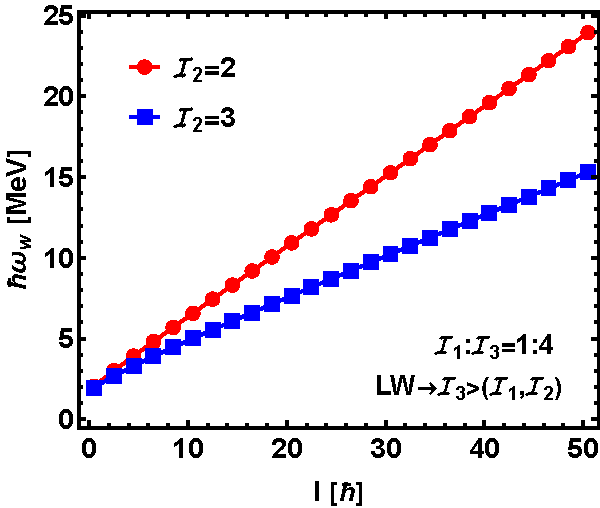
\includegraphics[width=0.49\textwidth]{Chapters/Figures/wobb_freq_oddA-LW.pdf}
    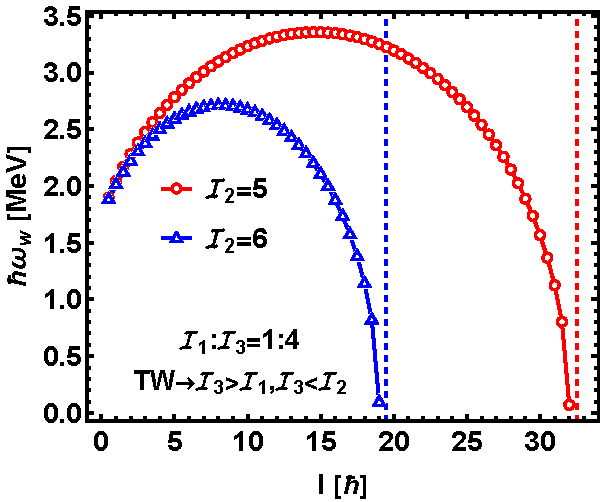
\includegraphics[width=0.49\textwidth]{Chapters/Figures/wobb_freq_oddA-TW.pdf}
    \caption{The wobbling frequency for an odd-$A$ nucleus, with the $\mathcal{Q}$'s a.m. $j=13/2$, coupled to the core $\mathscr{C}$. \textbf{Left:} The \emph{longitudinal wobbler} case with two sets of MOI, where only $\mathcal{I}_2$ differs. \textbf{Right:} The \emph{transverse wobbler} case with two sets of MOI, where only $\mathcal{I}_2$ is different. In both figures, the unit of $\mathcal{I}_k$ is $\hbar^2\text{MeV}^{-1}$. Note the vertical grid-lines in the right inset, signifying the critical angular momentum where the wobbling frequency reaches zero.}
    \label{wobbling-freq-oddA}
\end{figure}

In the same manner as for the simple wobbler, a geometrical representation for the coupling schemes in the longitudinal and transverse wobbling motion can be made in order to get a grasp on the alignments involved. As such, Fig. \ref{wobbling-oddA-geometry} shows these representations. Besides the wobbling regimes that emerge from a FA of the odd nucleon, two more wobbling modes can exist. Namely, for the yrast states (that is the lowest energy state of a given value of angular momentum $I$) and the \emph{excited state} of the odd-particle itself. When the a.m. of the odd nucleon starts to execute small precession around one of the principal axes of the triaxial core, then those excited states are regarded as \emph{signature partners} (since the de-alignment of the a.m. will cause the apparition of the favored and un-favored sequences, as described in Section \ref{section-ral-signature}). The yrast wobbling is simply regarded as a complete alignment of the odd-nucleon and core angular momenta with the $m$-axis, whose coupling scheme is similar to LW except that there is no precessional motion for the angular momenta. These two particular cases are graphically represented (in the same manner as for LW and TW) in Fig. \ref{wobbling-geometry-YRAST-SPB}.
\begin{figure}
    \centering
    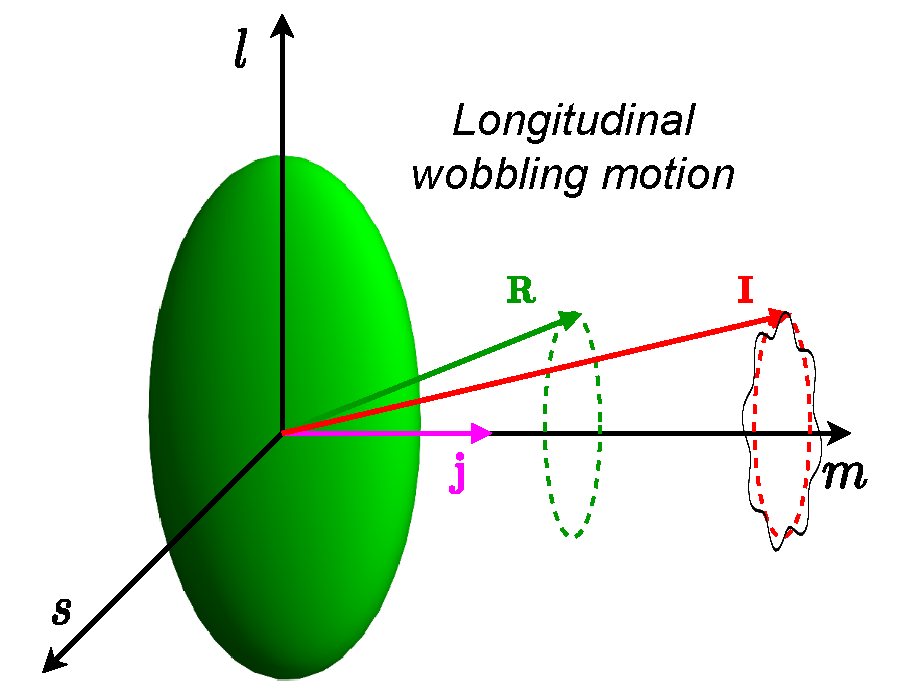
\includegraphics[scale=0.5]{Chapters/Figures/longitudinal_wobbler-schematic.pdf}
    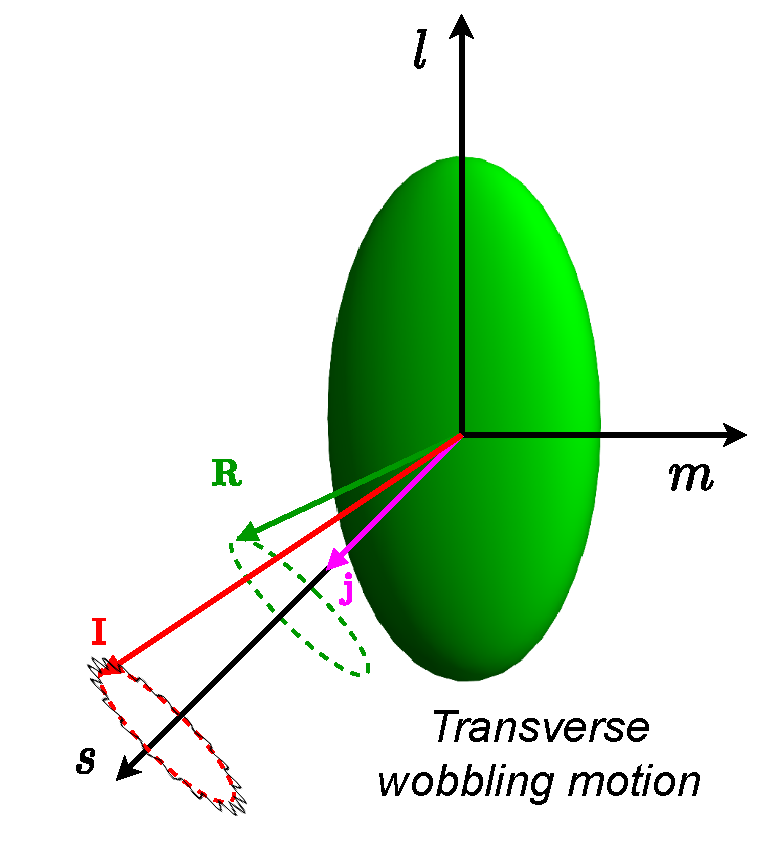
\includegraphics[scale=0.5]{Chapters/Figures/transverse_wobbler-schematic.pdf}
    \caption{Geometrical representation with the alignment scheme for a longitudinal wobbler and a transverse wobbler. The the a.m. vectors for the quasi-particle, the core, and the total system are represented by $\mathbf{j}_\mathcal{Q}$, $\mathbf{R}_\mathscr{C}$, and $\mathbf{I}$, respectively. Note that the precessional motion with oscillator-like behavior of $\mathbf{I}$ is illustrated with the encircled sine wave (black color). The resulting motion of the total a.m. will consist in a precessional cone that is properly depicted in Figs. \ref{advanced-quasiparticle-coupling-1}-\ref{advanced-quasiparticle-coupling-3}.}
    \label{wobbling-oddA-geometry}
\end{figure}
\begin{figure}
    \centering
    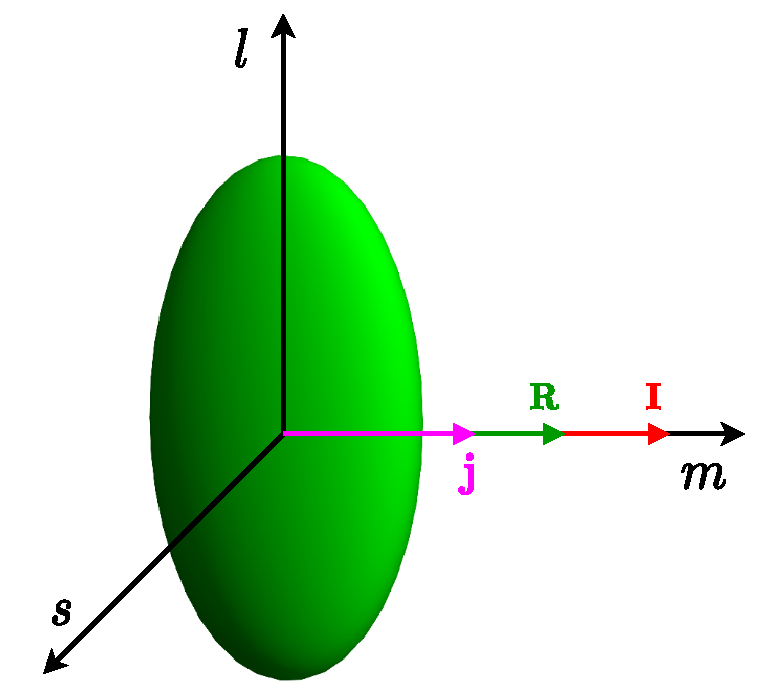
\includegraphics[scale=0.55]{Chapters/Figures/yrast_wobbler-schematic.pdf}
    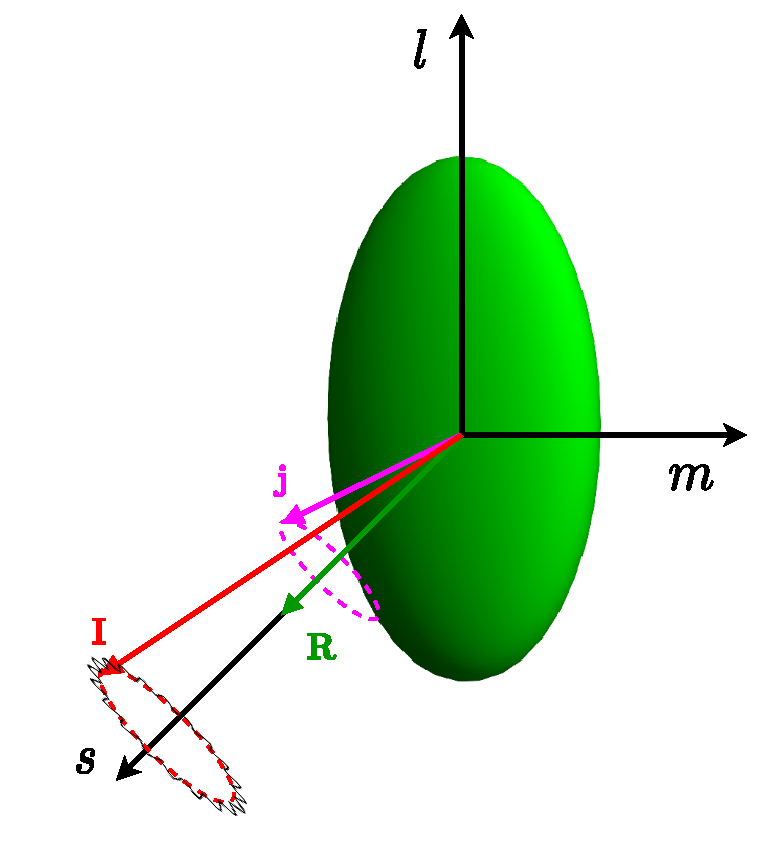
\includegraphics[scale=0.55]{Chapters/Figures/signaturePartner_wobbler-schematic.pdf}
    \caption{Geometrical representation with the alignment scheme for an yrast wobbling state and signature partner wobbling band. The the a.m. vectors for the quasi-particle, the core, and the total system are represented by by $\mathbf{j}_\mathcal{Q}$, $\mathbf{R}_\mathscr{C}$, and $\mathbf{I}$, respectively. Note that the precessional motion with oscillator-like behavior of $\mathbf{I}$ is illustrated with the encircled sine wave (black color). For the signature partner wobbling, the core's a.m. is aligned with one of the principal axes. The resulting motion of the total a.m. will consist in a precessional cone that is properly depicted in Figs. \ref{advanced-quasiparticle-coupling-1}-\ref{advanced-quasiparticle-coupling-3}.}
    \label{wobbling-geometry-YRAST-SPB}
\end{figure}

In this section, the collective motion specific to triaxial structures was treated for an odd-$A$ nucleus, starting from an initial rotor Hamiltonian, amended with a single-particle term. It was shown that based on the $\mathcal{Q}$+$\mathscr{C}$ coupling scheme, two scenarios might emerge, and the geometrical representation for both of them is illustrated in Fig. \ref{wobbling-oddA-geometry} together with the workflow diagrams depicted in Figs. \ref{advanced-quasiparticle-coupling-1}-\ref{advanced-quasiparticle-coupling-3}. The LW regime is characterized by an increase in wobbling energy with spin, while the opposite is true for TW regime. Moreover, within the HA and keeping the quasi-particle's a.m. fixed along a principal axes, the expression for $\hat{H}$ was obtained via Eq. \ref{hamiltonian-qtr-FA}, which is quite close to the case of even-even nuclei (see Eq. \ref{general-rotor-ham-evenA}). The wobbling frequencies were also expressed (see Eqs. \ref{wobbling-frequency-odd-A-inertiaParams} - \ref{wobbling-frequency-odd-A-MOI}). The quantitative analysis of the wobbling frequency in both wobbling regimes was performed in Fig. \ref{wobbling-freq-oddA}, and moreover, the reduced inertia factor $\mathscr{A}_3$ introduced in Eq. \ref{reduced-inertia-parameter-A3} is studied w.r.t. change of total spin $I$.

Concluding, the wobbling phenomenon was properly described through a quantitative analysis of different observables of interest (rotational frequency, wobbling frequency, wobbling energy, MOI, and so on) for even-even nuclei and also for odd-$A$ nuclei, showing multiple sets of results. In the next chapter, the introduction of the `core'-framework of this research can be finally done, starting from the initial assumptions, and reaching the important results and features that emerge from the formalism.

\section{Wobbling Nuclei - A Complete Catalog}

In this section, an inventory of all the known wobbling nuclei will be made. It is worth mentioning that there are ongoing debates regarding the experimental measurements for some of these isotopes and their `validity' on wether wobbling is present or not. Any existing conjecture will be mentioned where needed. For each wobbler, the band structure, the deformation parameters, and other important observations will be emphasized. Knowing the deformation parameters, one can also categorize the isotopes within regions of \emph{normal deformation} (ND structures) or \emph{strong deformation} (SD structure).

Although WM was predicted theoretically more than 50 years ago by Bohr and Mottelson \cite{bohr1998nuclear}, the first experimental observation of this collective mode has been confirmed in 2001. Moreover, the predictions were initially made for even-even nuclei, but the first nucleus in which wobbling was identified is the odd-$A$ $^{163}$Lu \cite{odegaard2001evidence}. The advance in technological equipment that allows high resolution/precision measurements has been very persistent over the last two decades, resulting in more and more successful investigations of the nucleonic matter at very high angular momentum ($I\approx 50\hbar$ or even $I\approx 80\hbar$). In what follows, the known wobblers will be categorized based on the atomic mass $A$, while, in a final diagram, all the known isotopes will be mapped. The mapping procedure is another useful feature of this current research, since it provides an easy and quick way of visualizing the progress towards the wobbling spectroscopy in the field of nuclear physics. This also constitutes the incipient phase in the development of an \emph{online digital register} with the current nuclei that will provide even more data.

\subsection{Wobbling around A=100}

In this region, recent measurements show that $^\mathbf{105}$\textbf{Pd} \cite{timar2019experimental} has two rotational bands built as wobbling excitations. The odd quasi-particle is a neutron from the $h_{11/2}$ orbital, coupling to the even-even core. The $\mathcal{Q}+\mathscr{C}$ coupling in which the valence nucleon is a neutron represents a rare example across the nuclide chart. The even-even nucleus $^\mathbf{112}$\textbf{Ru} \cite{hamilton2010super} is also reportedly to have three wobbling bands (one yrast and two excited), showing that from the three isotopes $^{108,110,112}$Ru, this one is the only one exhibiting a stable triaxial shape. Moreover, this isotope represents one of the few examples of collective excitations emerging from even-mass nuclei. Additionally, some measurements on $^\mathbf{114}$\textbf{Pd} \cite{luo2013triaxial}, which is an isotone of the previous nucleus, show that the two bands with different signature ($\alpha=0$ and $\alpha=1$) have similar behavior with the ones from $^{112}$Ru (the excitation energies as function of angular momentum varies in the same fashion). However, the determination of mixing ratios and transition probabilities between levels was not possible, so the interpretation of these structures as wobbling bands cannot be fully ascertained \cite{lv2022experimental}.

\subsection{Wobbling around A=130}

Chakraborty et al. \cite{chakraborty2020multiphonon} identified some wobbling bands in the odd-$A$ $^\mathbf{127}$\textbf{Xe} isotope. The collective states are built on the odd $\nu h_{11/2}$ nucleon configuration, leading to the apparition of four bands, two decoupled bands (i.e., favored $\alpha=-1/2$ and un-favored $\alpha=1/2$) with zero-phonon number, and two excited ($n_w=1,2$) wobbling bands. The wobbling energies (as defined in previous sections) are increasing functions with angular momentum, indicating that $^{127}$Xe would behave as a longitudinal wobbler. Another presumably longitudinal wobbler is the nucleus $^\mathbf{133}$\textbf{La} with two wobbling bands $n_w=0$ and $n_w=1$ \cite{biswas2019longitudinal} that exhibit enhanced $E2$ transition probabilities and mixing ratios (which are considered hallmarks of wobbling motion). The neighboring nucleus $^\mathbf{135}$\textbf{Pr} was also investigated, and three wobbling bands are reported (the yrast and $n_w=1$ bands in \cite{matta2017transverse} and $n_w=2$ in \cite{sensharma2019two}). The remarking feature is that the wobbling energies for this isotope are decreasing functions of spin, meaning that the TW regime prevails. The transition from LW to TW between $^{133}$La and its close neighbor $^{135}$Pr is a remarking feature of this elusive phenomenon. An explanation of this change in motion will be discussed at the end of the section. Although there is inconclusive evidence regarding transition probabilities and mixing ratios \cite{ma1990competing,kaur2014high}, the yrast band from $^\mathbf{131}$\textbf{Ba} which built on the $\mathcal{Q}_h$ neutron ($h_{11/2}$) can have an excited wobbling band, with negative parity spins ranging from $13/2$ to $29/2$ \cite{petrache_2018}. If precise measurements for the transition probabilities $B(E2)$ will show enhanced values, then indication of transverse wobbling will be conclusive.

The isotope $^\mathbf{133}$\textbf{Ba} is another odd-mass nucleus in which three wobbling bands have been identified by Devi et al. \cite{devi2021observation} very recently. Besides the excited $n_w=1$ and $n_w=2$, the yrast $n_w=0$ band has a signature partner band. All four bands have negative parity states. Devi et al. found out that the wobbling energies and the alignment behave quite similarly to $^{135}$Pr, concluding that this nucleus is a transverse wobbler. The remarking characteristic of the wobbling motion in this nucleus is that so far, this is the first wobbler in which a hole-like particle $\mathcal{Q}_h$ couples to the core $\mathscr{C}$, stabilizing the total system to a non-axial shape. Indeed, the odd $h_{11/2}$ neutron aligns itself with the long axis of the core, causing the TW regime to appear.

Within the last couple of years, a set of measurements brought light upon several even-even wobblers, although more precise measurements are required for ascribing triaxiality to this collective phenomenon with certainty. An example is the isotope that was studied in Section \ref{ba-130-numerical-calculations}, namely $^\mathbf{130}$\textbf{Ba} \cite{petrache2019diversity,chen2019transverse,wang2020two}. This nucleus exhibits wobbling via the coupling of two protons $(h_{11/2})^2$ with $\mathscr{C}$. Since the measurements of the transition probabilities show enhanced values, typical to wobbling, the isotope is regarded as a clear transverse wobbler. Petrache et al. \cite{petrache2016transverse} also discovered transverse wobbling within some nuclei that were recently studied in terms of chiral-like structures (i.e., the Nd and Ce isotopes). Indeed, in their research, $^\mathbf{134}$\textbf{Ce} has two wobbling bands (yrast and one excited) with the configuration of 2-$\mathcal{Q}_h$ with neutrons ($h_{11/2}$), while $^\mathbf{136}$\textbf{Nd} has two excited wobbling bands, both decaying out to the yrast sequence, built on a 2-$\mathcal{Q}_p$ configuration with the protons $(h_{11/2})^2$ coupling to $\mathscr{C}$. The isotope $^\mathbf{138}$\textbf{Nd} is also investigated by Petrache et al. \cite{petrache2012tilted} which could exhibit wobbling behavior, through one excited band that decays to the yrast band, with a configuration of two quasi-particles $\mathcal{Q}$ consisting in a proton-neutron pair.

\subsection{Wobbling around A=160}

A highly-aligned $\mathcal{Q}$ will favor a specific triaxial shape \cite{hamamoto1983intrinsic} given by the $j$-orbital itself. Moreover, the degree of shell filling will dictate a particular value for the triaxiality parameter $\gamma$. In turns out that for this proton, the favored triaxiality is around $\gamma=20^\circ$, meaning that PES calculations on strongly deformed triaxial structure will show stable minima around that $\gamma$-value. The wobbling excitations appear since only a small rotational energy is needed for building excited levels above the yrast line \cite{hamamoto2016interplay}.

Experimentally, this is the \emph{richest} region within the chart of nuclides characterized by wobbling motion. As mentioned at the start of the section, the first ever nucleus in which this phenomenon was recognized was $^\mathbf{163}$\textbf{Lu} \cite{odegaard2001evidence}. Therein, with the Euroball detector \cite{simpson1997euroball} array, a second \emph{strongly triaxial band} (TSD2) with familiar properties as the previous one (TSD1) was measured. Both bands were built on the configuration of a $\mathcal{Q}_p$ that is a proton in $i_{13/2}$ shell. In fact, along the $A\approx 160$ region, this \emph{intruder} will cause most of the triaxial structures to become enhanced and stable. One year later, a second excited wobbling band (TSD3) was confirmed as a wobbling band \cite{jensen2002evidence}, and the team recently ascribed TSD4 to wobbling excitations as well \cite{raduta2020towards}. The measurements indicate large quadrupole values, enhanced quadrupole transitions, and quantities such as alignment, dynamic moment of inertia, and excitation energies relative to a reference show similarities across each of the four bands, with magnitudes that are higher than other neighboring (coexisting) normal deformed structures \cite{jensen2004coexisting}. This is a clear indicator that stable triaxial structures exist in $^{163}$Lu. After this discovery, a large number of wobbling bands, appearing at large deformation parameters were identified in $^\mathbf{161}$\textbf{Lu} \cite{bringel2005evidence} (one excited wobbling band), $^\mathbf{165}$\textbf{Lu} \cite{schonwasser2003one} (two excited), $^\mathbf{167}$\textbf{Lu} \cite{amro2003wobbling} (one excited), and $^\mathbf{167}$\textbf{Ta} \cite{hartley2009wobbling} (one excited).

It is worth mentioning that the isotopes in this particular region have large spins, meaning that they are also rapidly rotating. When fast rotation occurs, both the core as well as the particle's a.m. will align with the intermediate axis, meaning that these wobblers behave as longitudinal wobblers. However, qualitatively, the wobbling energies have a decreasing trend with spin $I$, showing a transverse-like character. For the high-spin region, the wobbling mechanism is explained through a `top-on-top' model \cite{hamamoto2002wobbling,tanabe2006algebraic} (analogy with the classical asymmetric top).

\subsection{Wobbling around A=180}

A set of new measurements show some wobbling structures in the heavy-nuclei region. Namely, the $^\mathbf{183}$\textbf{Au} \cite{nandi2020first} nucleus and $^\mathbf{187}$\textbf{Au} \cite{sensharma2020longitudinal,sensharma2021wobbling}. In the former, two wobbling bands were identified, one built on a positive parity proton $i_{13/2}$ and one built on a negative parity proton $h_{9/2}$. The remarking feature of this nucleus is that even though both protons align perpendicular to the intermediate axis (showing a TW regime), the behavior of the wobbling energies show some decrease, Nandi et al. suspecting that these band represent the initial increasing part of wobbling energies in transverse wobbling bands. Therein, an interesting remark is raised, suggesting that the increasing/decreasing trend for wobbling energies must not be considered as the sole indicator for LW/TW regime (this discussion is also emphasized in a recent work done by the current team \cite{poenaru2021extensive1,poenaru2021extensive2}). The latter nucleus exhibits longitudinal wobbling motion, having one yrast band and one excited, and the yrast band has a signature partner. Both bands are built on the configuration of a proton from $h_{9/2}$ $j$-orbital, located at the middle of the shell, suggesting a LW behavior (since the $\mathcal{Q}$ will align its a.m. along the $m$-axis of the core).

The nuclei indexed here are the currently known wobblers (or `candidates') and in the following, a catalog that will also show important values such as the quadrupole deformation parameter, the triaxiality parameter, and quadrupole moments. Besides the graphical catalog with all the mentioned nuclei, some figures showing experimental wobbling energies are also illustrated, in order to get a grasp of the qualitative behavior of wobbling energies with increasing spin.  

\subsubsection*{The transition between wobbling regimes}

The already discussed isotopes $^{133}$La and $^{135}$Pr show an interesting phenomenon, where the former exhibits an increasing energy, while the latter (with only two extra nucleons) shows a decreasing trend. This rather `abrupt' change in the $\mathcal{Q}+\mathscr{C}$ coupling, (i.e., parallel alignment of $\mathcal{Q}$ with the core in the first case, and perpendicular alignment in the second) was explained by Biswas et al. \cite{biswas2019longitudinal}. Indeed, in both nuclei the $\mathcal{Q}_p$ ($h_{11/2}$ proton) is expected to align with the $s$-axis, such that the two isotones must exhibit transverse wobbling. But the situation can be understood in the following way: the $\mathcal{Q}_p$ in $^{135}$Pr aligns its a.m. with the short axis of the triaxial core and since the $m$-axis has the largest MOI, TW will arise. However, for $^{133}$La, besides the $h_{11/2}$ proton, an extra pair of protons (positive-parity) will align gradually with the $s$-axis of the triaxial density distribution. It is this additional alignment that increases the effective MOI of the short axis, which achieves a higher magnitude than the one along the $m$-axis. This re-arrangement will finally result in the LW behavior of the isotope.

The LW/TW behavior within the two nuclei can also be understood in terms of angular momentum behavior w.r.t. the rotational frequency (i.e., the backbending curves). For $^{133}$La, there is a rather constant and gradual increase in spin with the rotational frequency. On the other hand, $^{135}$Pr shows a strong backbend with increasing spin (although rather late). Additionally, both nuclei show rotation around the short axis close to the yrast line (since the proton will align its a.m. with that axis). The MOI of the $s$-axis for $^{135}$Pr is smaller than the one of the $m$-axis, and with increasing spin it becomes convenient to add more and more collective angular momentum on the $m$-axis since $\mathcal{I}_m>\mathcal{I}_s$. Consequently, the wobbling frequency will start to decrease with increasing spin and so does the final wobbling energy. Such a mechanism clearly leads to transverse regime. The ratio $\mathcal{I}_m$ to $\mathcal{I}_s$ is closer to $1$ for $^{133}$La, meaning that the medium axis is no longer preferred by the collective a.m., and the $s$-axis will start to gain more and more of it. The increase of collective a.m. along the short axis causes the wobbling frequency to increase with spin, which is specific to the longitudinal character. The evolution with rotational frequency of the total angular momentum in both nuclei can be seen in Fig. \ref{spin-vs-rotationalFreq-133-135}. Notice the gradual increase of the yrast band for $^{133}$La vs. the sharp backbend present in $^{135}$Pr.
\begin{figure}
    \begin{center}
        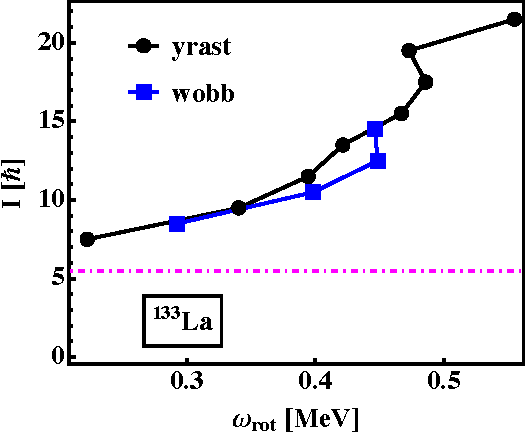
\includegraphics[width=0.49\textwidth]{Chapters/Figures/133La.pdf}
        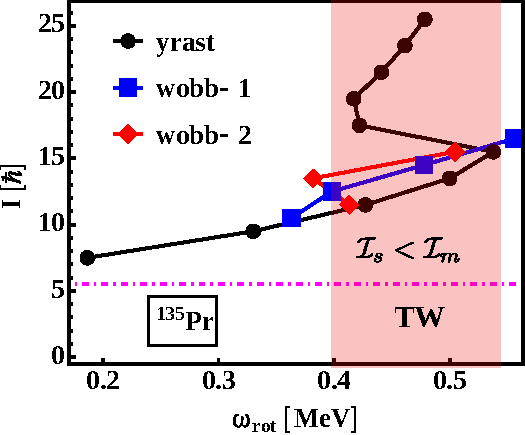
\includegraphics[width=0.49\textwidth]{Chapters/Figures/135Pd_edited.pdf}
        \caption{The angular momentum evolution with respect to the (experimental) rotational frequency $\omega_\text{rot}$ for $^{133}$La (\textbf{left}) and $^{135}$Pr (\textbf{right}). The backbending region for the latter nucleus is illustrated within the red color sector. Since the $s$-axis MOI is smaller, more and more collective a.m. will be added to this axis, causing a decrease in the wobbling frequency. The dotted magenta line represents the spin value of the odd proton.}
        \label{spin-vs-rotationalFreq-133-135}
    \end{center}
\end{figure}